\documentclass[a4paper]{article}

\usepackage{adjustbox}
\usepackage{algorithm}
\usepackage{algorithmic}
\usepackage{amsmath}
\usepackage{amssymb}
\usepackage{amsthm}
\usepackage{amsfonts}
\usepackage{afterpage}
\usepackage{blindtext}
\usepackage[font=footnotesize,labelfont=bf]{caption}
\usepackage{hyperref}
\usepackage[english]{babel}
\usepackage{bbm}
\usepackage{bigints}
\usepackage{bm}
\usepackage{cite}
\usepackage{color}
\usepackage{float}
\usepackage[left=2cm,right=2cm,top=2cm,bottom=2cm]{geometry}
\usepackage{graphicx}
\usepackage[utf8]{inputenc}
\usepackage{mathtools}
\usepackage{mdframed}
\usepackage{pgfplots} 
\usepackage{subfigure}
\usepackage{stmaryrd}
\usepackage{textcomp}
\usepackage{tikz}
\usepackage{url}
\renewcommand{\proofname}{Proof}
\theoremstyle{plain}
\newtheorem{monTheoNumrote}{Théorème}[section] % Environnement numéroté en fonction de la section
\newtheorem*{monTheoNonNumerote}{Théorème}  % Environnement non numéroté
\newtheorem{The}{Theorem}[section]
\newtheorem*{The*}{Theorem}
\newtheorem{Prop}{Proposition}[section]
\newtheorem*{Prop*}{Proposition} 
\newtheorem{Cor}{Corollary}[section]
\newtheorem*{Cor*}{Corollary}
\newtheorem{Conj}{Conjecture}[section]
\newtheorem{Lem}{Lemma}[section]
\renewcommand{\qed}{\unskip\nobreak\quad\qedsymbol}%
\numberwithin{equation}{section} % Numérote les équations section.numéro.
\theoremstyle{definition}
\newtheorem{Def}{Definition}[section]
\newtheorem{Rem}{Remark}[section]
\newtheorem*{Rem*}{Remark}
\newtheorem*{Lem*}{Lemma}
\newtheorem{Que}{Question}
\newcommand{\enstq}[2]{\left\{#1\mathrel{}\middle|\mathrel{}#2\right\}}
\newcommand{\Lp}[2]{L^#1(#2)}
\newcommand{\Sob}[3]{W^{#1,#2}(#3)}
\newcommand{\Rd}[0]{\mathbb{R}^d}
\newcommand{\RN}[0]{\mathbb{R}^N}
\newcommand{\Rn}[0]{\mathbb{R}^n}
\newcommand{\norm}[1]{\left\|#1\right\|}
\newcommand{\sinc}[0]{\textup{sinc}}
\newcommand{\functionDef}[5]{\begin{array}{lllll}
#1 & : & #2 & \longrightarrow & #3 \\
 & & #4 & \longmapsto &\displaystyle #5 \\
\end{array}}
\newcommand{\Theautorefname}{Theorem}
\newcommand{\Propautorefname}{Proposition}
\newcommand{\Corautorefname}{Corollary}
\newcommand{\Lemautorefname}{Lemma}
\newcommand{\Defautorefname}{Definition}
\newcommand{\N}{\mathbb{N}}
\newcommand{\Z}{\mathbb{Z}}
\newcommand{\D}{\mathbb{D}}
\newcommand{\R}{\mathbb{R}}
\newcommand{\A}{\mathcal{A}_{a,b}}
\newcommand{\Crad}{C^\infty_{c,rad}(B)}
\newcommand{\Lrad}{L^2_{rad}(B)}
\newcommand{\Lradab}{L^2_{rad}(\mathcal{A}_{a,b})}
\newcommand{\duality}[2]{\left\langle #1,#2\right\rangle}
\newcommand{\Hrad}{H^1_{rad}(B)}
\newcommand{\Hzrad}{H^1_{0,rad}(B)}
\newcommand{\rmin}{\delta_{\min}}
\newcommand{\rmax}{\delta_{\max}}
\newcommand{\corr}{\gamma}
\newcommand{\question}[1]{\begin{Que} \ 
#1
\end{Que}}
\newcommand{\abs}[1]{\left\lvert #1 \right\rvert}
\newcommand{\CL}[2]{\textup{CL}\left(\enstq{#1}{#2}\right)}
\newcommand{\Script}[1]{`\texttt{#1}`}
\newcommand{\espace}{\text{ }\qquad} 
\newcommand{\loc}{\text{loc}}
\newcommand{\SL}{\textup{SL}\hspace{1.5pt}}
\newcommand{\DL}{\textup{DL}\hspace{1.5pt}}
\newcommand{\fp}{\underset{\varepsilon \to 0}{\textup{f.p.}}}
\newcommand{\scalProd}[2]{\left(#1|#2\right)}
\newcommand{\toDo}[1]{{\color{red}#1}}
\newcommand{\bs}[1]{\boldsymbol{#1}}
\newcommand{\varInRange}[4]{(#1_{#2})_{#3 \leq #2 \leq #4}}
\newcommand{\from}{\colon}
\newcommand{\Cinf}{C^{\infty}}
\newcommand{\isdef}{\mathrel{\mathop:}=}
\newcommand{\defis}{=\mathrel{\mathop:}}

\renewcommand{\algorithmicrequire}{\textbf{Inputs:}}
\renewcommand{\algorithmicensure}{\textbf{Outputs:}}

\pgfplotsset{compat=1.13}


\title{Preconditionning the Helmholtz problem on curved arcs in dimension 2}
\author{Fran\c{c}ois Alouges and Martin Averseng\footnote{CMAP, Ecole polytechnique, Route de Saclay, 91128 Palaiseau Cedex.}}
\begin{document}
	\maketitle
	
	\begin{abstract}
	\end{abstract}
	
	\section{Introduction}
	The problem of preconditionning the linear systems coming from the discretization of integral equations
	has received considerable attention since two decades roughly. Among the possible strategies are the so-called 
	pseudo-differential preconditionner, whose analysis uses tools from pseudo-differential calculus \cite{Christiansen,Nedelec,Levadoux,DarbasAntoine}. Roughly speaking, if the original problem is written in the abstract way
	\begin{equation}
	\mathcal{L}u=f\,,
	\label{eq1}
	\end{equation}
	the strategy consists in findind a suitable operator $\mathcal{K}$ such
	that, when left mulitplying the (\ref{eq1}) by $\mathcal{K}$, one needs to solve
	\begin{equation}
	\mathcal{K}\mathcal{L}u=\mathcal{K}f\,.
	\end{equation}
	Now if $\mathcal{K}\mathcal{L}$ is a compact perturbation of the identity, the condition number of the discretized underlying
	system is independant of the chosen size of the mesh, leading to optimal convergence rate of the numerical methods used to solve the system.
	
	Several strategies, depending on the problem to solve have been studied in the literature \cite{} to propose such operators $\mathcal{K}$, that often turn out to be very effective in practice, when numerical applications are considered.
	However, all the preceding results and theories are limited to smooth domains and very little is known when the integral equation 
	is posed on domains with corners (in 2D), wedges or conical points (in 3D). One of the reason might be the fact that 
	pseudo-differential calculus is difficult to generalize on such manifolds, and more problematic, the underlying operators
	are difficult to analyze on such domains.
	
	Nevertheless, a program similar to those given on smooth manifold was proposed a few years ago \cite{Bruno,Nedelec,Jerez,Hiptmair} who tackled the problem of preconditionning the first or second layer potential
	for Laplace or Helmholtz equation in dimension 2 or 3 but for very particular domains: a straight and then curved segment in 2D and a unit disc in 3D.
	
	\toDo{finir l'intro et mettre le plan}
	
	The remainder of the paper focuses on the numerical solution of the integral equations \eqref{dirichletIntEq} and \eqref{NeumannIntEq} using Galerkin finite elements. Though this will not lead to spectral convergence as when using trigonometric polynomial, we aim to generalize our method to cases where the eigenvectors of the operators are not explicitly known. In the first section, we treat the two equations corresponding to the case $k=0$ and when $\Gamma$ is the segment. We introduce the same rescaled operators as in \cite{bruno2012second}. We derive a simple preconditioner for both integral equation in the form of the square root of the differential operators \eqref{cheb1} and \eqref{cheb2}, and verify its efficiency on numerical experiments using Galerkin discretization with piecewise polynomial finite elements. In the next section, we treat the general case using standard compact perturbation arguments, leading to a new preconditioner. Numerical tests are again provided.
	
	
	\section{The scattering problem in 2D}
	We focus here on the 2D case and consider the problem of the scattering of a wave by an open line. Let $\Gamma$ be a smooth non-intersecting open curve, and let $k \geq 0$ the wave number. We seek for a solution of the problem
	\begin{equation}
	-\Delta u - k^2 u = 0,  \text{ in } \R^2 \setminus \Gamma
	\label{Helmholtz}
	\end{equation}
	when one considers furthermore
	\begin{itemize}
		\item Dirichlet or Neumann boundary conditions, namely
		\begin{equation}
		u = u_D, \text{ on } \Gamma
		\label{Dirichlet}
		\end{equation}
		or
		\begin{equation}
		\dfrac{\partial u}{\partial n} = u_N  \text{ on } \Gamma 
		\label{Neumann}
		\end{equation}
		respectively.
		\item Suitable decay at infinity, given by the Sommerfeld condition
		\begin{equation}
		\dfrac{\partial u}{\partial r} - iku = o\left(\frac{1}{\sqrt{r}}\right)
		\label{Sommerfeld}
		\end{equation}
		with $r=|x|$ for $x\in \mathbb{R}^2$.
	\end{itemize}
	In the preceding equation $n$ stands for a smooth unit normal vector to $\Gamma$.
	
	Existence and uniqueness of solutions to the previous problems are guaranteed by the following theorem.
	\begin{The}(see e.g. \cite{stephan1984augmented,wendland1990hypersingular,monch1996numerical}) Assume $u_D \in H^{1/2}(\Gamma)$, and $u_N \in H^{-1/2}(\Gamma)$. Then problems (\ref{Helmholtz},\ref{Dirichlet},\ref{Sommerfeld}) and (\ref{Helmholtz},\ref{Neumann},\ref{Sommerfeld}) both possess a unique solution $u \in H^1_\textup{loc}(\R^2 \setminus \Gamma)$, which is of class $C^{\infty}$ outside $\Gamma$. Near the edges of the screen $\Gamma$, for the Dirichlet problem, the solution has an unbounded gradient, with for $x\in \gamma$
		\[\dfrac{\partial u}{\partial n}(x) = O\left(\frac{1}{\sqrt{d(x,\partial \Gamma)}}\right),\]
		while for the Neumann problem, one has \toDo{pas joli}
		\toDo{Qu'est-ce qui n'est pas joli exactement ? Je ne sais pas trop quoi changer.}
		\[u(x) = \sum_{i=1}^2 \alpha_i \sqrt{\rho_i}\chi_i + \psi\]
		where $\psi \in \tilde{H}^{3/2}(\Gamma)$. Here, $\chi_1$ and $\chi_2$ are two functions concentrated near each edge of the arc, $\rho_i$ is the distance between $x$ and the tip $i$, and $\alpha_i$ are two real numbers. 
	\end{The}
	
	For the definition of Sobolev spaces on smooth open curves, we follow
	\cite{mclean2000strongly} by considering any smooth closed curve $\tilde{\Gamma}$ containing $\Gamma$, and defining 
	\[H^s(\Gamma) = \enstq{U_{|\Gamma}}{ U \in H^s(\tilde{\Gamma}) }.\]
	
	Obviously, this definition does not depend on the particular choice of the closed curve $\tilde{\Gamma}$ containing $\Gamma$. Moreover,
	\[\tilde{H}^s(\Gamma) = \enstq{u \in H^s(\Gamma)}{\tilde{u} \in H^s(\tilde{\Gamma})}\]
	where $\tilde{u}$ denotes the extension by zero of $u$ on $\tilde{\Gamma}$.
	
	\paragraph{Single-layer potential}  
	The solution to the preceding problems can be expressed through integral formulations. Namely, we define for any smooth function $\lambda$ defined on $\Gamma$ the single-layer potential $\mathcal{S}_k$  by 
	\begin{equation}
	\mathcal{S}_k\lambda(x) = \int_{\Gamma}G_k(x-y)\lambda(y)d\sigma(y)
	\label{defSk}
	\end{equation}
	where $G_k$ is the Green's function defined by 
	\begin{equation}
	\left\{
	\begin{aligned}
	G_0(z) &= -\dfrac{1}{2\pi} \ln \abs{z}, && \text{ if } k= 0,\\
	G_k(z) &= \frac{i}{4}H_0(k|z|), && \text{ if } k > 0,
	\end{aligned} \right.
	\end{equation} 
	for $x\in \mathbb{R}^2\setminus \Gamma$. Here $H^{(0)}_k$ is the Hankel function of the first kind. It is well known that $\mathcal{S}_k$ can be extended to a continuous mapping 
	\[\mathcal{S}_k : \tilde{H}^{-1/2}(\Gamma) \to H^1_{\text{loc}}(\R^2)\] 
	and calling $S_k = \gamma \mathcal{S}_k$ where $\gamma$ is the trace operator on $\Gamma$, we may write the solution
	$u$ of the Dirichlet problem (\ref{Helmholtz},\ref{Dirichlet},\ref{Sommerfeld}) as
	\begin{equation}
	u = \mathcal{S}_k \lambda
	\end{equation}
	where $\lambda \in \tilde{H}^{-1/2}(\Gamma)$ solves
	\begin{equation}
	S_k \lambda = u_D\,.
	\label{Sklambda}
	\end{equation}
	
	\paragraph{Double-layer and hypersingular potentials}
	Similarly, we introduce the double layer potential $\mathcal{D}_k$ by 
	\[\mathcal{D}_k \mu(x) = \int_{\Gamma} n(y) \cdot \nabla G_k(x-y) \mu(y) d\sigma(y).\]
	for any smooth function $\mu$ defined on $\gamma$. This time, $\mathcal{D}_k$ extends to a continuous mapping 
	\[\mathcal{D}_k : \tilde{H}^{1/2}(\Gamma) \to H^{1}_{\text{loc}}(\R^2 \setminus \Gamma)\]
	and the function $\mathcal{D}_k \mu$ has a jump across $\Gamma$. We define 
	\[D_k \mu  = \lbrace\mathcal{D}_k \mu \rbrace\]
	where $\lbrace u \rbrace$ denotes the average value of $u$ on each side of $\Gamma$. $D_k$ is then a continuous operator from $\tilde{H}^{1/2}(\Gamma)$ to $H^{1/2}(\Gamma)$. 
	
	It is well-known that the normal derivative of $\mathcal{D}_k\mu$ is continuous across $\Gamma$, allowing us to define the hypersingular operator $N_k = \partial_n \mathcal{D}_k$. This operator admits the representation for $x\in \Gamma$
	\begin{equation}
		N_k \mu = \lim_{\varepsilon \to 0^+} \int_{\Gamma} n(y) \cdot \nabla G(x + \varepsilon n(x) - y) \mu(y) d\sigma(y).
		\label{defNk}
	\end{equation}
	The kernel of this operator has a non-integrable singularity, but numerical calculations are made possible by the following formula, valid for smooth functions $\mu$ and $\nu$ that vanish at the extremities of $\Gamma$: 
	\begin{equation}
		\duality{N_k \mu}{\nu} = \int_{\Gamma\times \Gamma} G_k(x-y) \mu'(x) \nu'(y) - k^2 G_k(x,y) \mu(x) \nu(y) n(x) \cdot n(y) d\sigma(x) d\sigma(y)\,.
		\label{NkenfonctiondeSk}
	\end{equation}
	It is also known that $N_k$ maps $\tilde{H}^{1/2}(\Gamma)$ to $H^{-1/2}(\Gamma)$ continuously, and that the solution $u$ to the Neumann problem (\ref{Helmholtz},\ref{Neumann},\ref{Sommerfeld}) can be written as
	\begin{equation}
	u = \mathcal{D}_k \mu
	\end{equation}
	where $\mu \in \tilde{H}^{1/2}(\Gamma)$ solves
	\begin{equation}
	N_k \mu = u_N\,.
	\label{Nkmu}
	\end{equation}  
	
	\section{The case of Laplace equation on a flat segment}
	
	In this section, we restrict our attention to the case where $\Gamma$ is the open segment $(-1,1) \times \{0\}$, and $k=0$. We study the properties of the equations 
	\[S\lambda = -u_D\]
	and 
	\[N\mu = u_N\]
	and show their invertibility in a range of Sobolev-like spaces. This problem has been already considered thoroughly, both
	in terms of analytical and numerical properties in the literature (see for instance \cite{,,,}), and it turns out that the Chebyshev polynomials of first and second kind play a very important role. However, we go further compared to the literature
	by constructing a functional framework close to Sobolev spaces, based on Chebyshev polynomials that
	allows us to give a complete framework for the existence and uniqueness of the solutions to the preceding equations, as well as
	new preconditioners.
	
	\subsection{Analytic setting}
	Chebyshev polynomials of first and second kinds are respectively given by 
	\[T_n(x) = \cos(n \arccos(x)),\]
	and 
	\[U_n(x) = \dfrac{\sin((n+1) \arccos(x))}{\sqrt{1 - x^2}}\,.\]
	
	We let $\omega(x) = \sqrt{1-x^2}$. We also denote by $\omega$ the operator $u(x) \mapsto \omega(x)u(x)$. Moreover, let $\partial_x$ the derivation operator, the Chebyshev polynomials satisfy
	the ordinary differential equations
	\begin{eqnarray*}
		(1-x^2)T_n'' -xT_n' +n^2T_n =0\,\mbox{ and }(1-x^2)U_n'' -3xU_n' +n(n+2)U_n =0
	\end{eqnarray*}
	that we rewrite under the form
	\begin{eqnarray}
	(\omega\partial_x)^2 T_n &=& -n^2T_n\,, \label{cheb1}\\
	(\partial_x\omega)^2 U_n &=& -(n+1)^2U_n\, .\label{cheb2}
	\end{eqnarray}
	(Notice that by $(\partial_x\omega)^2 U_n$ we mean $\partial_x(\omega \partial_x (\omega U_n))$.)
	As we shall see, the preceding equations are crucial in our analysis. 
	
	Both $T_n$ and $U_n$ are polynomials of degree $n$, and form orthogonal families respectively of the Hilbert spaces 
	$$L^2_{\frac{1}{\omega}} \isdef \enstq{u \in L^1_\textup{loc}(-1,1)} {\int_{-1}^{1} \dfrac{f^2(x)}{\sqrt{1 - x^2} }dx< + \infty}$$
	and 
	$$L^2_{\omega} \isdef \enstq{u \in L^1_\textup{loc}(-1,1)} {\int_{-1}^{1} {f^2(x)}{\sqrt{1 - x^2} }dx< + \infty}.$$
	We denote by $\duality{\cdot}{\cdot}_\frac{1}{\omega}$ and $\duality{\cdot}{\cdot}_\omega$ the inner products in $L^2_{\frac{1}{\omega}}$ and $L^2_{\omega}$ respectively.
	Chebyshev polynomials also satisfy
	\begin{equation}
	\int_{-1}^1  \dfrac{T_n(x)T_m(x)}{\sqrt{1 - x^2} }dx = \left\{
	\begin{array}{l}
	0 \mbox{ if } n\ne m\\
	\pi \mbox{ if } m=n=0\\
	\pi/2 \mbox{ otherwise}
	\end{array} 
	\right.
	\end{equation}
	and
	\begin{equation}
	\int_{-1}^1  U_n(x)U_m(x)\sqrt{1 - x^2} dx = \left\{
	\begin{array}{l}
	0 \mbox{ if } n\ne m\\
	\pi/2 \mbox{ otherwise}
	\end{array} 
	\right.
	\end{equation}
	which provides us with the so-called Fourier-Chebyshev decomposition. Any
	$u\in L^2_{\frac{1}{\omega}}$ can be decomposed through the first kind Chebyshev series 
	\begin{equation}
	u(x) = \sum_{n=0}^{+\infty} \hat{u}_n T_n(x)
	\label{FCseries}
	\end{equation}
	where the Fourier-Chebyshev coefficients $\hat{u}_n$ are given by 
	\[ \hat{u}_n \isdef \begin{cases}
	\dfrac{2}{\pi}\displaystyle\int_{-1}^{1} \dfrac{u(x) T_n(x)}{\sqrt{1-x^2}}dx & \text{ if } n \neq 0\,,\\
	\dfrac{1}{\pi}\displaystyle\int_{-1}^{1} \dfrac{u(x)}{\sqrt{1-x^2}}dx & \text{ otherwise,}\\
	\end{cases}\]
	and satisfy the Parseval equality
	\[ \int_{-1}^{1} \frac{u^2(x)}{\sqrt{1-x^2}} dx =  \frac{\pi \hat{u}_0^2}{2} + \pi\sum_{n=1}^{+\infty}\hat{u}_n^2\,.\]
	When $u$ is furthermore a smooth function, the series \eqref{FCseries} converges uniformly to $u$. Similarly, any 
	function $v\in L^2_{\omega}$ can be decomposed along the $U_n$ as
	\[ v(x) = \sum_{n=0}^{+\infty} \check{v}_n U_n(x)\]
	where the coefficients $\check{v}_n$ are given by 
	\[ \check{v}_n \isdef 
	\dfrac{2}{\pi}\displaystyle\int_{-1}^{1} v(x) U_n(x)\sqrt{1-x^2}dx  \]
	with the Parseval identity
	\[ \int_{-1}^{1} v^2(x)\sqrt{1-x^2} dx =  \frac{\pi}{2} \sum_{n=0}^{+\infty}\check{v}_n^2\,.\]
	The preceding analysis can be generalized to define Sobolev-like spaces. 
	\begin{Def}
		For all $s \geq 0$, we may define 
		\[T^s = \enstq{ u \in L^2_\frac{1}{\omega}}{ \sum_{n=0}^{+\infty}(1+n^2)^s \hat{u}_n^2 < + \infty}.\]
		This is a Hilbert space for the scalar product
		\[\duality{u}{v}_{T^s} = \frac{\pi}{2}\hat{u}_0 \hat{v}_0 + \pi\sum_{n=1}^{+\infty}(1+n^2)^s\hat{u}_n \hat{v}_n.\]
		We also define a semi-norm 
		\[\abs{u}_{T^s} \isdef \sum_{n = 1}^{+ \infty}n^{2s} \abs{\hat{u}_n}^2.\]
		We denote by $T^{\infty}$ the Fr\'echet space $T^{\infty} \isdef \displaystyle\cap_{s \in \R} T^s$, and by $T^{-\infty}$ the set of continuous linear forms on $T^{\infty}$. For $l \in T^{-\infty}$, we note $\hat{l}_n = l(T_n)$, so that for $u \in T^{\infty}$, 
		\[l(u) = \frac{\pi}{2}\hat{l}_0 \hat{u}_0 + \pi \sum_{n=1}^{+\infty} \hat{l}_n \hat{u}_n\,.\] 
		
		We choose to identify the dual of $L^2_\frac{1}{\omega}$ to itself using the previous bilinear form.  With this identification, any element of $T^s$ with $s \geq 0$ can also be seen as an element of $T^{-\infty}$.  
		Furthermore, the space $T^{-s}$ can be defined for all $s \geq 0$ as
		\[T^{-s} = \enstq{ u \in T^{-\infty}}{ \sum_{n=0}^{+\infty}{(1 + n^2)^{-s} \hat{u}_n^2} < \infty}.\]
		Using the preceding identification $T^{-s}$ becomes the dual of $T^s$. Obviously, for any real $s$, if $u \in T^s$, the sequence of polynomials 
		\[S_N(x) = \sum_{n=0}^{N} \hat{u}_n T_n(x)\]
		converges to $u$ in $T^s$. Therefore, the space $C^{\infty}([-1,1])$ is dense in $T^s$ for all $s \in \R$. For $s < t$, the inclusion $T^s \subset T^t$ is compact.
	\end{Def}
	\noindent In a similar fashion, we define the following spaces:
	\begin{Def}
		For all $s \geq 0$, we set
		\[U^s = \enstq{u \in L^2_\omega}{ \sum_{n=0}^{+\infty} (1 + n^2)^s\check{u}_n^2}.\]
		We extend as before the definition to negative indices by setting $U^{-s}$ to be the dual of $U^s$ for $s\geq 0$. 
	\end{Def}
	\noindent We now give some basic properties of these spaces:
	\begin{Lem}
		\label{inclusionsTsUs}
		For all real $s$, $T^s \subset U^s$ and for all $s > 1/2$, $U^s \subset T^{s-1}$.
	\end{Lem}
	\begin{proof}
		The first property is immediate once it has been noticed that for $n \geq 2$, $T_n(x) = \frac{1}{2}\left(U_n - U_{n-2}\right)$, while $T_0 = U_0$ and $T_1 = \frac{U_ 1}{2}$. The second comes from the expressions
		\[U_{2n} = 2\sum_{j = 0}^n T_{2j} - 1, \quad U_{2n+1} = 2\sum_{j=0}^n T_{2j+1}.\]
		When $u \in U^{s}$ for $s > 1/2$, the series $\sum \abs{\check{u}_n}$ is converging, allowing to identify $u$ to a function in $T^{-\infty}$, with 
		\[\hat{u}_{0} = \sum_{n=0}^{+ \infty} \check{u}_{2n}, \quad  \hat{u}_j = 2\sum_{n=0}^{+\infty} \check{u}_{j + 2n} \textup{ for } j \geq 1.\]
		Since $u \in U^s$, $(1+n^2)^{s/2} \abs{\check{u}}$ is in $l^2$ and by continuity of the adjoint of the Cesàro operator in $l^2$, the sequence $r_n \isdef \left( \sum_{k=n}^{+ \infty} (1+k^2)^{\frac{s-1}{2}} \abs{\check{u}_k}\right)_n$ is in $l^2$. But
		\begin{eqnarray*}
			\norm{u}_{T^{s-1}}^2 &=& \sum_{n=0}^{+ \infty} (1 + n^2)^{s-1} \abs{\hat{u}_n}^2\\ 
			&\leq& 4\sum_{n=0}^{+\infty}(1+n^2)^{s-1} \left(\sum_{k=n}^{+\infty} \abs{\check{u}_k}\right)^2 \\
			&\leq& 4\sum_{n=0}^{+ \infty}\left(\sum_{k=n}^{+\infty}(1+k^2)^{\frac{s-1}{2}} \abs{\check{u}_k})\right)^2.\\
			&=& 4\norm{r_n}^2_{l^2}.
		\end{eqnarray*}	
	\end{proof}
	One immediate consequence is that $T^{\infty} = U^{\infty}$.  Moreover, we have the following result:
	\begin{Lem}
		\[T^{\infty} = C^{\infty}([-1,1])\,.\]
		\label{LemTinfCinf}
	\end{Lem}
	\begin{proof}
		If $u \in C^{\infty}([-1,1])$, then we can obtain by induction using integration by parts and \eqref{cheb1}, that for any $k \in \N$
		\[\hat{u}_n = \frac{(-1)^k}{n^{2k}} \int_{-1}^{1} \dfrac{(\omega\partial_x)^{2k} u(x) T_n(x)}{\omega(x)}dx.\]
		Noting that $(\omega \partial_x)^2 = (1-x^2)\partial_x^2 - x \partial_ x$, this proves that $C^{\infty}([-1,1]) \subset T^{\infty}$. 
		
		To prove the converse inclusion, first notice that, by normal convergence of the series, $T^{\infty} \subset C^0([-1,1]) $. Now, let $u \in T^{\infty}$, it suffices to show that $u' \in T^{\infty}$ and apply an induction argument. Applying term by term differentiation, we obtain
		\[u'(x) = \sum_{n=1}^{+\infty} n u_n U_{n-1}(x).\] 
		Therefore, $u'$ is in $U^{\infty} = T^{\infty}$. 
	\end{proof}
	\begin{Prop}
		If $\psi$ is a $C^{\infty}$ function on $[-1,1]$, then the operator
		\[ u(t) \mapsto \psi(t) u(t)\]
		is of order $0$, and for any $s \in \R$, 
		\[ \norm{\psi u}_{T^s} \leq C2^{\abs{s}/2}\norm{u}_{T^s} \norm{\psi}_{T^{\abs{s}+1}}.\]
		where $C$ is independent of $\psi$ and $s$. 
		\begin{proof}
			Let $u \in T^s$, we rewrite $u$ as 
			\[ u = \sum_{n = -\infty}^{+ \infty}u_n'T_n\]
			where for $n< 0$ we define $T_{n} = T_{\abs{n}}$, and with 
			\[u_n' = \begin{cases}
			u_0 & \text{ if } n = 0\\
			\frac{u_{\abs{n}}}{2} & \text{ otherwise.}
			\end{cases}\]
			We apply the same idea to $\psi$, and using $T_m T_n = T_{m+n} + T_{m-n}$, 
			\[\psi u = \sum_{m,n} u'_n \psi'_m (T_{m+n} + T_{m-n}) = \sum_{m} \left(\sum_{n}u'_n(\psi'_{n + m} + \psi'_{n - m})\right) T_m\]
			that is, by parity
			\[\psi u = 2\sum_{m,n} u'_m \psi'_{m-n} T_{n}\]
			Using Peetre's inequality, we have 
			\[(1 + n^2)^{s/2}\abs{(\psi u)_n} \leq 2^{\abs{s}/2+1}\sum_{m}(1 + m^2)^{s/2} \abs{u'_m}  (1 + |n-m|^2)^{\abs{s/2}} \abs{\psi'_{n-m}} \]
			and by Young's inequality with $r = 2, p = 2, q = 1$, 
			\[\norm{\psi u}_s^2 \leq 2^{\abs{s}+2}\norm{u}_s^2 \sum_{m=-\infty}^{+\infty} (1 + m^2)^{\abs{s}/2}\abs{\psi'_m} \]		
			The last sum is finite because $\psi \in T^{\infty}$ and
			\[\sum_{m=-\infty}^{\infty}(1 + m^2)^{\abs{s}/2} \abs{\psi'_m} \leq \left(\sum_{m = -\infty}^{+ \infty} \frac{1}{1 + m^2} \right)\sum_{m=-\infty}^{+\infty} (1 + m^2)^{\abs{s}+1}\abs{\psi'}_m^2.\]
		\end{proof}
		\begin{Lem}
			Let $g(x,y)$ the kernel of an integral operator of order $\alpha \in \R$ in the spaces $T^s$, that is,
			\[G : u \mapsto \int_{-1}^{1} \frac{g(x,y) u(y)}{\omega(y)}dy\]
			is continuous from $T^s$ to $T^{s + \alpha}$ for all $s$. Let $R(x,y)$ a $C^{\infty}$ function. Then the operator 
			\[K : \int_{-1}^{1} \frac{g(x,y) R(x,y) u(y)}{\omega(y)}dy\]
			is of order $\alpha$. 
		\end{Lem}
		\begin{proof}
			Since $R$ is in $C^{\infty}$, we can write 
			\begin{equation}
			R(x,y) = \sum_{m,n} r_{m,n} T_m(x) T_n(y)
			\label{sommenormalementcv}
			\end{equation}
			where $r_{m,n}$ satisfies for all $s,t \in \R$, 
			\[\sum_{m,n} (1 + m^2)^s (1 + n^2)^t\abs{r_{m,n}}^2 < +\infty.\] 
			For each $m,n$, the operator $T_m G T_n$ defined by 
			\[ T_m G T_n u = T_m(x) \int_{-1}^{1} \dfrac{G(x,y) T_n(y)u(y)}{\omega(y)}dy\]
			is in $L(T^s,T^{s+\alpha}$ by the previous lemma, with 	\[\norm{T_m G T_n}_{T^s \to T^{s+\alpha}} \leq C 2^{\abs{s} + \abs{s + \alpha}}(1 + n^2)^{\abs{s}+1}(1 + m^2)^{\abs{s+ \alpha} + 1}.\]
			thus, the series in \eqref{sommenormalementcv} is normally convergent in $L(T^s, T^{s + \alpha})$, which proves the claim. 
		\end{proof}
	\end{Prop}
	\begin{Lem}
		\label{LemInjectionsContinues}
		For all $\varepsilon >0$, if $u \in T^{\frac{1}{2} + \varepsilon}$, then $u$ is continuous and there exists a constant $C$ such that for all $x \in [-1,1]$,
		\[ \abs{u(x)} \leq C \norm{u}_{T^{1/2 + \varepsilon}}.\]	
		Similarly, if $u \in U^{3/2 + \varepsilon}$, then $u$ is continuous and 
		\[ \abs{u(x)} \leq C \norm{u}_{U^{3/2 + \varepsilon}}.\]
		\begin{proof}
			We write 
			\[\abs{u(x)} \leq \sum_{n = 0}^{+ \infty} \abs{\hat{u}_n}\]
			since for all $n$, $\norm{T_n}_{L^\infty} = 1$. Cauchy-Schwarz's inequality then yields
			\[\abs{u(x)} \leq \sqrt{\sum_{n= 0}^{+ \infty} \frac{1}{(1+ n^2)^{\frac{1}{2}+ \varepsilon}}} \norm{u}_{T^{\frac{1}{2} + \varepsilon}}.\]
			For the second statement, we use the inclusion $U^{s} \subset T^{s-1}$ valid for $s > 1/2$, as established in \autoref{inclusionsTsUs}. 
		\end{proof}	
	\end{Lem}
	\begin{Lem}
		We have $L^2_\omega = \frac{1}{\omega}L^2_\frac{1}{\omega}$ and the pointwise multiplication by $\frac{1}{\omega}$ defines an bijective isometry from $L^2_\frac{1}{\omega}$ to $L^2_\omega$ with inverse $\omega$. 
		\label{isometrie}
	\end{Lem}
	\begin{Lem}
		For all real $s$, the operator $\partial_x$ can be extended into a continuous map from $T^{s+1}$ to $U^{s}$ as
		\[ \duality{\partial_x u}{v}_{\omega} \isdef -\duality{u}{\omega \partial_x \omega v}_{\frac{1}{\omega}}.\] 
		For all real $s$, the  operator $\omega \partial_x \omega$ can be extended into a continuous operator from $U^{s+1} \to T^{s}$ as
		\[\duality{\omega \partial_x \omega u}{v}_\frac{1}{\omega} \isdef -\duality{u}{\partial_x v}_\omega.\]
		\begin{proof}
			First, note that if $v \in T^{\infty}$, then  $\omega \partial_x \omega v = (1-x^2)v' - xv \in T^{\infty}$. The definition of $\partial_x$ is thus correct. The claimed continuity  is an immediate consequence of 
			\[\omega \partial_x \omega U_n = -(n+1) T_{n+1}.\]
			The second assertion comes from $T_n' = nU_{n-1}$. 
		\end{proof}
	\end{Lem}
	\noindent The following corollary will be used in our Galerkin analysis:
	\begin{Cor}
		\label{corDxT2T0}
		The operator $\partial_x$ is continuous from $T^{s+2}$ to $T^s$ for all $s > -1/2 $ and from $U^{s+2}$ to $U^s$ for all $s > - 3/2$.
	\end{Cor}
	\begin{proof}
		For the first case we use $\partial_x$ is continuous from $T^{s+2}$ to $U^{s+1}$ and then the identity is continuous from $U^{s+1}$ to $T^s$. For the second, we use the same arguments in the reverse order. 
	\end{proof}
	We now provide a characterization of the spaces $T^s$ and $U^s$. For this, we need the following result:
	\begin{Cor}
		\label{omegadxetdxomga}
		The operator $\omega \partial_x$ defined on $T^{\infty}$ as 
		\[\omega \partial_x u = \omega u'\]
		has a continuous extension from $T^1$ to $T^0$. Similarly, the operator $\partial_x \omega$ has a continuous extension from $U^1$ to $U^0$. 
		\begin{proof}
			For the first part, we use the fact that $\partial_x$ is continuous from $T^1$ to $U^0$, and, by \autoref{isometrie}, $\omega$ is continuous from $U^0$ to $T^0$. 
			For the second part, we use the fact that $\omega \partial_x \omega$ is continuous from $U^1$ to $T^0$, and from the same lemma, the multiplication by $\frac{1}{\omega}$ is continuous from $T^0$ to $U^0$. 
		\end{proof}
	\end{Cor}
	For a function $u$ defined on $[a,b]$, we denote by $\tilde{u}$ the function defined on $[\theta_a,\theta_b] \isdef [\arccos(a),\arccos(b)]$ as
	\[ \tilde{u}(\theta) = u(\cos(\theta))\]
	and by $Vu$ the function defined as 
	\[Vu(\theta) \isdef \sin(\theta) \tilde{u}(\theta).\]
	We then have the following characterization:
	\begin{The}
		$u \in T^n \iff \tilde{u} \textup{ is even and } \tilde{u}\in H^n(-\pi,\pi)$. In this case, 
		\[ \norm{u}_{T_n}\sim \norm{\tilde{u}}_{H^n}, \abs{u}_{T^n} \sim \abs{\tilde{u}}_{H^n}.\]
		Similarly, $u \in U^n \iff Vu \textup{ is odd and } Vu \in H^n(-\pi,\pi)$. In this case, 
		\[\norm{u}_{U_n} \sim \abs{Vu}_{H^n}.\]	
		If $ u \in T^n$, $(\omega \partial_x)^n u$ is in $L^2_\frac{1}{\omega}$ and 
		\[ \abs{u}_{T^n}^2 \sim \int_{-1}^{1} \frac{((\omega \partial_x)^n u)^2}{\omega}\]
		\noindent If $u \in U^n$, $(\partial_x \omega)^n \in L^2_\omega$ and 
		\[ \norm{u}_{U_n} = \int_{-1}^{1}\omega ((\partial_x \omega)^n u)^2\]
		\label{thmChar}
	\end{The}
	\begin{proof}
		The first two equivalences stem from the fact that 
		\[\hat{u}_n = \frac{1}{\pi}\int_{-\pi}^{\pi} \tilde{u}(\theta) \cos(n \theta), \check{u}_n = \frac{1}{\pi} \int_{-\pi}^{\pi} Vu(\theta) \sin((n+1)\theta)d\theta,\]
		which can be verified by using the change of variables $x = \cos\theta$ in the definitions of $\hat{u}_n$ and $\check{u}_n$. 
		Now, let us show that if $ u \in T^n$, then $(\omega \partial_x)^n$ is in $L^2_\frac{1}{\omega}$. The operator $(\omega \partial_x)^2$ is continuous from $T^s$ to $T^{s-2}$ for all real $s$ which implies the result if $n$ is even. If $n$ is odd, say $n = 2k + 1$, we write $(\omega \partial_x)((\omega \partial_x)^{2})^k$, and conclude using \autoref{omegadxetdxomga}.
		The same kind of proof also shows that if $u \in U^n$, $(\partial_x \omega )^nu \in L^2_\omega$.
		The rest of the proof can be performed by computing the quantities for functions in $T^{\infty}$, perform integrations by part and conclude with the density of $C^{\infty}$ in $T^s$ and $U^s$. 
	\end{proof}
	\begin{Def}
		If $A : T^{\infty} \to T^{-\infty}$ can be extended into a continuous operator from $T^{s}$ to $T^{s + p}$ for any $s \in \R$, we shall say that it is of order $p$. When an operator is of order $p$ for all $p \in \N$, we call it a smoothing operator. When $A$ and $B$ are such that there exists a smoothing operator $R$ such that 
		\[A = B + R,\]
		we write $A = B \textup{  mod  }  T^{\infty}$.
	\end{Def}
	
	
	
	
	%\begin{Prop}
	%	\toDo{Pas sûr que ce soit utile, ni même vrai...}
	%	For $m \in \N$, the norm on $T^m_\omega$ is equivalent to 
	%	\[\norm{u}_m^2 = \int_{-1}^{1}\frac{u^2}{\omega} + \int_{-1}^1 \dfrac{\abs{(\omega \partial_x)^m u}^2}{\omega}\]
	%\end{Prop}
	
	%As well as a decomposition in Chebyshev polynomials of the first kind, any function can be expanded in polynomials of the second kind: 
	%\[u(x) = \sum_{n=0}^{+\infty} \bar{u}_n U_n(x)\]
	%where 
	%\[\bar{u}_n = \dfrac{2}{\pi}\int_{-1}^{1}\sqrt{1 - x^2}u(x)U_n(x)dx.\]
	%

	
	\subsection{Single layer equation}
	
	In this section we focus on the equation $S\lambda = g$, that is we seek $\lambda \in \tilde{H}^{-1/2}$ such that 
	\begin{equation}
	-\frac{1}{2\pi}\int_{-1}^{1} \log|x-y| \lambda(y) = -g(x), \quad \forall x\in (-1,1)\,.\label{Slambda}
	\end{equation} 
	
	This equation is sometimes called ``Symm's integral equation'' and its resolution has received a lot of attention in the 1990's. Numerical methods, using both collocation and Galerkin have been presented and analyzed \cite{atkinson1991numerical,yan1988integral,yan1990cosine,sloan1992collocation,yan1989mesh}. 
	
	%The solution is connected to the exterior Dirichlet problem for the Laplace operator, but attention must be paid when the solution $\lambda$ obtained does not satisfy $\duality{1}{\lambda}_\Gamma = 0$: in this case, $\textup{SL}\lambda$ is not a bounded solution of the Dirichlet problem. See \cite{atkinson1991numerical} for a link with the logarithmic capacity of the line and how we recover the bounded solution from the solution of \eqref{Slambda}.
	
	Our analysis lies on the following formula. For a proof, see for example \cite{mason2002chebyshev} Theorem 9.2. Note that this is also the main ingredient in \cite{bruno2012second}.
	
	%
	%\paragraph{Autre idée de présentation.}
	%We first start with a commutation result
	%
	%\toDo{Commencer par le truc connu. Et en fait c'est normal. Balancer ensuite la commutation. Dire que ça n'a pas été remarqué. }
	%
	%\begin{Prop}
	%	Commutation de $S_\omega$ et $(\omega \partial_x)^2$. 
	%\end{Prop}
	%Exploitation en terme de vp. Dire qu'on a deux opérateurs avec spectre discret. (L'un est compact dans $L^2_\frac{1}{\omega}$, (sans preuve pour l'instant).
	%
	\begin{Prop}
		\[ -\frac{1}{2\pi}\int_{-1}^{1} \frac{\ln|x-y|}{\sqrt{1 - y^2}}T_n(y)dy = s_n T_n(x)\]
		where
		\[s_n \isdef \begin{cases}
		\dfrac{\ln(2)}{2} & \text{if } n=0\\
		\dfrac{1}{2n} & \text{otherwise}.
		\end{cases}\]
		\label{STn}
	\end{Prop}
	An equivalent statement, giving a rather beautiful decomposition, can be found in \cite{jerez2012explicit}, and also \cite{urzua2014optimal}. The proof in \cite{jerez2012explicit} is different from that of \cite{mason2002chebyshev}.
	\begin{The}(See Theorem 4.4 in \cite{jerez2012explicit})	
		\label{decompLnKernelTn}
		For a given $x \in (-1,1)$, the logarithmic kernel admits the following expansion 
		\[ \ln|x-y| = -\ln(2) - \sum_{n=1}^{+\infty} \frac{2}{n}T_n(x)T_n(y)\]
		where the convergence of the series is understood in $L^2_\frac{1}{\omega}((-1,1)^2)$.
	\end{The}
	
	Using the decomposition of $g$ and of the logarithmic kernel on the basis $T_n$, we see that the solution $\lambda$ to equation \eqref{Slambda} admits the following expansion 
	\begin{equation}
		\lambda(x) = \frac{1}{\sqrt{1-x^2}}\sum_{n=0}^{+ \infty} \frac{\hat{g}_n}{s_n} T_n(x).
		\label{expansionLambda}
	\end{equation}
	We deduce the following well-known fact:
	\begin{Cor}
		\label{CorSingularity}
		If the data $g$ is in $C^{\infty}([-1,1])$, the solution $\lambda$ to the equation 
		\[S\lambda = g\]
		is of the form 
		\[\lambda = \dfrac{\alpha}{\sqrt{1-x^2}}\]
		with $\alpha \in C^{\infty}([-1,1])$.  
		\toDo{[FA]Peut-etre mettre un poil d'explication en plus (pourquoi la s\'erie cv dans $C^\infty$ par exemple)}\\
		\toDo{J'inclus cette preuve pour expliquer, ça suffit ?:}
		\begin{proof}
			Let $\alpha = \sqrt{1 - x^2}\lambda$ where $\lambda$ is the solution of $S\lambda = g$ with $g \in C^{\infty}([-1,1])$. 
			\autoref{LemTinfCinf} implies that $g \in T^{\infty}$, and by equation \eqref{expansionLambda}, 
			\[ \hat{\alpha}_n = \frac{\hat{g}_n}{s_n},\]
			so $\alpha$ also  belongs to $T^{\infty} = C^{\infty}([-1,1])$. 
		\end{proof}
	\end{Cor}
	
	
	We follow \cite{bruno2012second} by noticing that the behavior in $\frac{1}{\sqrt{1-x^2}}$ is consistent with the expected singularity near the edges and introduce the weighted single layer operator as the operator that appeared in Proposition \ref{STn}.
	\begin{Def}(See \cite{bruno2012second}) 
		Let $S_\omega$ be the weighted single layer operator defined by
		\[\opFromTo{S_\omega}{\alpha \in \Cinf([-1,1])}{-\dfrac{1}{2\pi}}{\int_{-1}^1\dfrac{\ln|x-y|}{\omega(y)} \alpha(y)dy}\]
	\end{Def}
	\noindent We also recall that the operator $(\omega\partial_x)^2$ is defined by \[\opFromTo{(\omega\partial_x)^2}{\alpha \in \Cinf([-1,1])}{(1-x^2)\alpha''(x) - x \alpha'(x)}.\]
	
	The action of these operators on $T^{\infty}$ is easy to analyze using \eqref{cheb1} and \autoref{STn}. By density of $T^{\infty}$ in $T^s$ for all $s$, we get:
	\begin{Prop}
		The operator $S_\omega$ is a self-adjoint, positive definite operator, and defines a continuous bijection from $T^{s}$ to $T^{s+1}$ for all real $s$. In particular, $S_\omega$ is of order $1$ and is compact in $T^s$. 
		Similarly, for any $s \in \R$, the operator $-(\omega \partial_x)^2$ is positive, self-adjoint, and of order $-2$. 
	\end{Prop}
	\begin{proof}
		It suffices to remark that if $u=\sum_{n=0}^\infty \hat{u}_n T_n \in T^s$, then
		\[S_\omega u = \frac{\ln(2)}{2} \hat{u}_0 T_0 +  \sum_{n=1}^\infty \frac{\hat{u}_n}{2n} T_n\]
		while
		\[-(\omega \partial_x)^2 u = \sum_{n=0}^\infty n^2\hat{u}_n T_n \,.\]
	\end{proof}
	\noindent To obtain the solution of \eqref{Slambda}, we can thus solve 
	\begin{equation}
		S_\omega \alpha = -u_D,
		\label{Somegaalpha}
	\end{equation}
	and let $\lambda = \frac{\alpha}{\omega}$.  
	The following two lemmas show that the solution to the Symm's integral equation in the usual Sobolev spaces can be recovered from the solution to $S_\omega \alpha = g$ in the spaces $T^s$. 
	\begin{Lem}
		\label{LemmaT-1/2}
		We have $\tilde{H}^{-1/2}(-1,1) = \frac{1}{\omega}T^{-1/2}$ and for all $u \in \tilde{H}^{-1/2}(-1,1)$,
		\[\norm{u}_{\tilde{H}^{-1/2}} \sim \norm{\omega u}_{T^{-1/2}}.\] 
	\end{Lem}
	
	\begin{proof}
		Since the logarithmic capacity of the segment is $\frac{1}{4}$, the operator $S$ is positive and bounded from below on $\tilde{H}^{-1/2}(-1,1)$, (see \cite{mclean2000strongly} chap. 8). Therefore the norm on $\tilde{H}^{-1/2}(-1,1)$ is equivalent to 
		\[\norm{u}_{\tilde{H}^{-1/2}} \sim \sqrt{\duality{Su}{u}}.\]
		On the other hand, it is obvious that if $\alpha\in T^{-1/2}$
		\[ \norm{\alpha}_{T^{-1/2}} \sim \sqrt{\duality{S_\omega \alpha}{\alpha}_\omega}.\]
		It remains to notice that for $\alpha=\omega u$, the two duality products coincide.
	\end{proof}
	
	\begin{Lem} Similarly,
		\[H^{1/2}(-1,1) = T^{1/2}\]
		and for $u \in H^{1/2}(-1,1)$ we have
		\[\norm{u}_{H^{1/2}} \sim \norm{u}_{T^{1/2}}\,.\]
		\label{LemmaT1/2}
	\end{Lem}	
	\begin{proof}
		We know that $(H^{1/2})'(-1,1) =  \tilde{H}^{-1/2}(-1,1)$ (cf \cite{mclean1986spectral} chap. 3), and therefore
		\[\norm{u}_{H^{\frac{1}{2}}} = \sup_{ v\neq 0} \dfrac{\duality{u}{v}}{\norm{v}_{\tilde{H}^{-\frac{1}{2}}}}\,.\]
		According to the previous lemma, for all $v\in \tilde{H}^{-\frac{1}{2}}$, the function $\alpha = \omega v$ is in $T^{-1/2}$, and $\norm{ v}_{\tilde{H}^{-1/2}} \sim \norm{\alpha}_{T^{-1/2}}$, while $\duality{u}{v} = \duality{u}{\alpha}_\omega$. Thus 
		\[\norm{u}_{H^{1/2}} \sim \sup_{\alpha \neq 0} \dfrac{\duality{u}{\alpha}_\omega}{\norm{\alpha}_{T^{-1/2}}}\]
		The last quantity is the $T^{1/2}$ norm of $u$ since $T^{1/2}$ is identified to the dual of $T^{-1/2}$ for $\duality{\cdot}{\cdot}_\omega$. 
	\end{proof}
	
	We are now in a position to find the inverse of $S_\omega$. An explicit inverse has already been appeared in the literature. In 
	particular, in \cite{jerez2011variational,urzua2014optimal}, explicit variational forms for this inverse operator are derived rigorously. (A similar method is also employed in the recent paper \cite{hiptmair2017closed} in $\R^3$ for the case of the unit disk.) We just state here the following formal decomposition:
	\[\dfrac{d^2}{dxdy}\log\frac{M(x,y)}{|x-y|^2} = \frac{-1+xy}{2|x-y|^2} = \sum_{n=1}^{+ \infty} n T_n(x)T_n(y)\]
	with 
	$M(x,y) = \frac{1}{2}\left((y-x)^2 + (\omega(x) + \omega(y))^2\right) $.
	\toDo{Et $T_0$?}\\
	\toDo{Hum je pense qu'il n'y pas de $T_0$ parce qu'on a des dérivées qui tuent le terme constant ici.}
	
	However, using the preceding analysis, we have an alternative way of defining this exact inverse, which leads to an 
	operator in the form of a square root. To state the next result, we define the operator $\pi_{0}$ as the $L^2_{1/\omega}$ 
	orthogonal projector on $T_0$. Namely 
	\[\pi_0 \alpha(x)  = \frac{1}{\pi} \int_{-1}^{1}\frac{\alpha(y)}{\omega(y)}dy\,.\]
	The preceding definition can be extended to $u \in T^s$ for any $s \in \R$ by setting $\pi_0 u$ as the solution of
	\[\left\{
	\begin{array}{l}\duality{\alpha-\pi_0 \alpha}{T_0}_{\frac{1}{\omega}} = 0\,,\\
	\pi_0\alpha\in \mbox{Span}(T_0)\,,
	\end{array}
	\right.\]
	since $T_0\in T^\infty$. Of course, $\pi_0$ is a smoothing operator. 
	
	\begin{The}
		\label{TheSdx2S}
		The operators $S_\omega$, $-(\omega\partial_x)^2$, and $\pi_0$ commute and satisfy
		\begin{equation}
		S_{\omega}\left(-(\omega\partial_x)^2 + \frac{1}{\ln(2)^2} \pi_0 \right)S_{\omega} = \frac{I}{4}\,.
		\label{Sdx2S}
		\end{equation}
	\end{The}
	\begin{proof}
		The Chebyshev polynomials $(T_n)$ are a common Hilbert basis of eigenvectors for the three operators $S\omega$, $-(\omega \partial_x)^2$ and $\pi_0$, so they all commute on $T^{-\infty}$. 
		Moreover, one has using \autoref{STn}, equation \eqref{cheb1} and the definition of $\pi_0$
		\[ S_\omega T_n =\frac{1}{2n}T_n\,,\,\, \pi_0 T_n = 0 \mbox{ and } -(\omega\partial_x)^2T_n = n^2 T_n \mbox{ if } n\ne 0\,,\]
		while
		\[ S_\omega T_0 = \frac{\ln(2)}{2} T_0\,,\,\, \pi_0 T_0 = T_0 \mbox{ and } -(\omega\partial_x)^2T_0 = 0 \mbox{ otherwise.}\]
		Equation \eqref{Sdx2S} follows from the fact that $(T_n)$ is a Hilbert basis of $T^{-\infty}$.
	 \end{proof}
	
	\begin{Rem} A direct proof of the commutation of $S_\omega$ and $-(\omega\partial_x)^2$ can be done. We give it in the 
		more general case of Helmholtz equation (see \autoref{Commutations}).
	\end{Rem}	
	From the preceding formula, we can extract the explicit inverse of $S_\omega$ in terms of the square root of the inner operator.
	\begin{Def}
		Let an operator $A : T^s \to T^{s + 2p}$ such that 
		\[AT_n = a_n T_n\]
		with $a_n \geq 0$. We define $\sqrt{A} T^s \to T^{s + p}$ as the operator satisfying 
		\[\sqrt{A}T_n = \sqrt{a_n} T_n.\]
	\end{Def}
	
	\begin{Cor}
		The inverse of $S_\omega$ can be equivalently expressed as 
		\begin{equation}
		S_{\omega}^{-1} = 2\sqrt{-(\omega \partial_x)^2 + \frac{1}{\ln(2)^2}\pi_0}\,.
		\end{equation}
	\end{Cor}
	
	The last result shows that $\sqrt{-(\omega \partial_x)^2}$ and $S_\omega$ can be thought as inverse operators (modulo constant terms) and that, at the very least, $\sqrt{-(\omega \partial_x)^2}$ can be used as a preconditioner for $S_\omega$. Indeed, $2\sqrt{-(\omega \partial_x)^2}S_\omega$ is a compact perturbation of identity. This makes a clear link with the approximation of the Dirichlet to Neumann map proposed in \cite{antoine2007generalized} in terms of a square root operator. The link will be even clearer when Helmholtz equation will be considered. Compared to the former formula, the proposed preconditionner only contains the weight $\omega$, which makes it very attractive for numerical implementation.
	
	\subsection{Hypersingular equation} 
	
	We now turn our attention to the equation 
	
	\begin{equation}
	N\mu = g
	\label{Nmu}
	\end{equation} 
	
	Similarly to the previous section and following again the idea of \cite{bruno2012second}, we consider a redcaled version of the hypersingular operator $N_\omega \isdef N \omega$ defined by
	
	\[N_\omega \mu = \lim_{\varepsilon\to 0}\int_{-1}^{1} n(y)\cdot\nabla G(x + \varepsilon n(x) - y) \sqrt{1-y^2} dy\]
	Analogous to the previous section, we can get the solution to \eqref{Nmu} by solving 
	\begin{equation}
	N_\omega \beta = u_N,
	\label{Nomegabeta}
	\end{equation}
	and letting $\mu = \omega \beta$. 
	We show that $N_\omega$ can also be analyzed in our functional framework, using now the spaces $U^s$. 
	\begin{Lem}
		\label{lemIPP}
		For any $\beta$, $\beta'$, one has 
		\[\duality{N_\omega \beta}{ \beta'}_\omega = \duality{S_\omega \omega \partial_x \omega \beta}{\omega \partial_x \omega \beta'}_\frac{1}{\omega}.\]
		\begin{proof}
			It is sufficient to show this formula for $\beta$ and $\beta'$ in $U^{\infty}$ by density. Indeed, for such $\beta, \beta'$, both sides of the identity define continuous bilinear forms on $T^{\infty}$. We use the well-known integration by part formula
			\[\duality{N u}{v} = \duality{S\partial_x u}{\partial_x v},\]
			valid when $u$ and $v$ vanish at the extremities of the segment (see for example \cite{bruno2012second}). 
			For a smooth $\beta$, we thus have
			\[ \duality{N (\omega \beta)}{ (\omega \beta')} = \duality{S \partial_x(\omega \beta)}{\partial_x (\omega \beta')}\] 
			which obviously implies the announced identity. 
		\end{proof}
	\end{Lem}
	\begin{Prop}
		$N_\omega$ is a positive definite, self-adjoint operator continuous from $U^s$ to $U^{s-1}$ for all real $s$. For all $n \in \N$, we have 
		\[N_\omega U_n = \frac{n+1}{2}U_n.\]
		Moreover, $-(\partial_x\omega)^2$ is also positive definite of order $2$.
		\label{NUn}
	\end{Prop}
	\toDo{Mettre une preuve ou une reference.}
	\begin{proof}
		\toDo{Voici une preuve:}\\
		From identity $T_{n+1}' = (n+1)U_n$ and Equation $\eqref{cheb1}$ we obtain
		\begin{equation*}
		\omega \partial_x \omega U_n = -(n+1) T_{n+1}.
		\end{equation*}
		Therefore, by \autoref{lemIPP}
		\begin{eqnarray*}
			\duality{N_\omega U_m}{U_n}_\omega & = & (n+1)(m+1)\duality{S_\omega T_{m+1}}{T_{n+1}}_\frac{1}{\omega}\\
			&=& \delta_{m=n} \frac{n+1}{2}.	
		\end{eqnarray*}
	The fact that $-(\partial_x \omega)^2$ is self-adjoint positive definite of order $2$ is a consequence of Equation \eqref{cheb2}.
	\end{proof}
	
	\noindent As a consequence, we have the following result:
	\begin{The} The operators $N_\omega$ and $-(\partial_x \omega)^2$ commute and 
		\[-N_\omega (\partial_x \omega)^{-2} N_{\omega} = \frac{I}{4}\,.\]
		The inverse of $N_\omega$ is therefore 
		\begin{equation}
		N_\omega^{-1} = 2\sqrt{-(\partial_x \omega)^{-2}}\,.
		\end{equation}
	\end{The}
	
	Like before, we have the following link between $U^{-1/2}$, $U^{1/2}$ and the usual Sobolev spaces. 
	\begin{Lem} The following identities hold, 
		\[\omega U^{1/2} = \tilde{H}^{1/2}(-1,1),\]
		\[ U^{-1/2} = H^{-1/2}(-1,1),\]
		with 
		\[\norm{\omega u}_{\tilde{H}^{1/2}} \sim \norm{u}_{U^{1/2}},\quad \norm{u}_{U^{-1/2}} \sim \norm{u}_{H^{-1/2}}.\]
		\label{lemU12H12}
	\end{Lem}
	\begin{proof} It suffices to remark that 
		\[ \norm{\omega u}_{\tilde{H}^{1/2}} \sim \sqrt{\duality{N\omega u}{\omega u}} = \sqrt{\duality{N_\omega u}{u}_\omega} \sim \norm{u}_{U^{1/2}}\,.\]
		The second equality follows from the same calculations that were done in Lemma \ref{LemmaT1/2},, as well as the norm equivalence. 
	\end{proof}
	
	
	In \cite{bruno2012second}, it is shown that $N_\omega S_\omega$ and $S_\omega N_\omega$ are order zero operators with a spectrum concentrated around $\frac{1}{4}$, which can be exploited for preconditioning purposes. 
	
	Analogously to the previous, one can also derive the formal expansions as in \cite{jerez2012explicit}
	\[\frac{1}{(x-y)^2} = \sum_{n=0}^{+\infty} 2(n+1)U_n(x)U_n(y)\,,\]
	that lead, by applying for $(\partial_x\omega)^{-2}$ on both sides, to the following explicit kernel for the inverse of $N_\omega$:
	\[\ln\left(\dfrac{(y-x)^2 + (\omega(x) + \omega(y))^2}{2|x-y|}\right) = \sum_{n=0}^{+\infty} \dfrac{2 U_n(x) U_n(y)}{n+1}.\]


\subsection{Galerkin analysis}


In this section, we describe and analyze a new Galerkin scheme to solve the integral equations \eqref{Slambda} and \eqref{Nmu}. Standard discretization on a uniform mesh with piecewise polynomial trial functions leads to very poor rates of convergences (see for example \cite[Chap. 4, ]{sauter2011boundary} and subsequent remark). Several methods have been developed to remedy this problem. One can for example enrich the trial space with special singular functions, refine the mesh near the segment tips, (h-BEM) or increase the polynomial order in the trial space. The combination of the last two methods, known as h-p BEM, can achieve an exponential rate of convergence with respect to the dimension of the trial space, see \cite{postell1990h} and references therein. Spectral methods, involving trigonometric polynomials have also been analyzed for example \cite{bruno2012second}, and some results exist for piecewise linear functions in the collocation setting \cite{costabel1988convergence}. 

Here, we describe a simple Galerkin scheme using piecewise affine functions on an adapted mesh, that is both stable and easy to implement. Our analysis shows that the usual rates of convergence one would obtain with smooth closed boundary with smooth solution, are recovered thanks to this new analytic setting. The orders of convergence are stated in \autoref{theOrdreCVDirichlet} and \autoref{theOrdreCVNeumann}. 

In what follows, we introduce a discretization of the segment $[-1,1]$ as $-1 = x_0 < x_1 < \cdots < x_N = 1$, and let $\theta_i \isdef \arccos(x_i)$. We define the parameter $h$ of the discretization as 
\[ h \isdef \min_{i=0\cdots N-1} \abs{\theta_{i+1} - \theta_{i}}.\]
In practice, one should use a mesh for which $\abs{\theta_i - \theta_{i+1}}$ is constant. This turns out to be analog to a graded mesh with the grading parameter set to $2$, that is, near the edge, the width of the $i-th$ interval is approximately $(ih)^2$. In comparison, in the h-BEM method with $p=1$ polynomial order, this would only lead to a convergence in $O(h)$ (cf. \cite[Theorem 1.3]{postell1990h}).

\subsubsection{Dirichlet problem}

In this section, we present the method to compute a numerical approximation of the solution $\lambda$ of \eqref{Slambda}. To achieve it, we use a variational formulation of \eqref{Somegaalpha} to compute an approximation $\alpha_h$ of $\alpha$, and set $\lambda_h = \frac{\alpha_h}{\omega}$. Let $V_h$ the Galerkin space of (discontinuous) piecewise affine functions with breakpoints at $x_i$. Let $\alpha_h$ the unique solution in $V_h$ to
\[ \duality{S_\omega \alpha_h}{\alpha_h'}_\frac{1}{\omega} = -\duality{u_D}{\alpha_h'}_\frac{1}{\omega}, \quad \forall \alpha_h' \in V_h.\]
We shall prove the following result:
\begin{The}
	If the data $u_D$ is in $T^{s+1}$ for some $-1/2 \leq s \leq 2$, then there holds:
	\[ \norm{\lambda - \lambda_h}_{\tilde{H}^{-1/2}} \leq C h^{s+1/2} \norm{u_D}_{T^{s+1}}.\]
	\label{theOrdreCVDirichlet}
\end{The}
In particular, when $u_D$ is smooth, it belongs to $T^{\infty}$ so the rate of convergence is $h^{5/2}$.
\noindent We start by proving an equivalent of Céa's lemma: 
\begin{Lem}
	\label{CeaDir}
	There exists a constant $C$ such that 
	\[\norm{\alpha - \alpha_h}_{T^{-1/2}} \leq C \inf_{{\alpha}_h' \in V_h}\norm{\alpha - {\alpha}_h'}_{T^{-1/2}}\]
	\begin{proof}
		 In view of the properties of $S_\omega$ stated in \autoref{STn}, we have the equivalent norm 
		 \[\norm{\alpha - \alpha_h}_{T^{-1/2}}^2 \leq C \duality{S_\omega(\alpha - \alpha_h)}{\alpha-\alpha_h}.\] 
		 Since $\duality{S_\omega \alpha}{\alpha_h'} = \duality{S_\omega \alpha_h}{\alpha_h'} = -\duality{u_D}{\alpha_h'}$ for all $\alpha_h' \in V_h$, we deduce 
		 \[\norm{\alpha - \alpha_h}_{T^{-1/2}}^2 \leq \duality{S_\omega (\alpha - \alpha_h)}{\alpha - \alpha'_h}, \quad \forall \alpha'_h \in V_N.\]
		 By duality
		 \[\norm{\alpha - \alpha_h}_{T^{-1/2}}^2 \leq C \norm{S_\omega(\alpha - \alpha_h)}_{T^{1/2}}\norm{\alpha - \alpha'_h}_{T^{-1/2}}\]
		 which gives the desired result after using the continuity of $S_\omega$ from $T^{-1/2}$ to $T^{1/2}$. 
	\end{proof}
\end{Lem}
From this we can derive the rate of convergence for $\alpha_h$ to the true solution $\alpha$. We use the $L^2_\frac{1}{\omega}$ orthonormal projection $\mathbbm{P}_h$ on $V_h$, which satisfies the following properties:
\begin{Lem}
	For any function $u$, 
	\[\norm{(\textup{I} - \mathbbm{P}_h)u}_{L^2_\frac{1}{\omega}} \leq C\norm{u}_{L^{2}_\frac{1}{\omega}},\]
	\[\norm{(\textup{I} - \mathbbm{P}_h)u}_{L^2_\frac{1}{\omega}}  \leq C h^2 \norm{u}_{T_2}.\]
	\label{PhT0T2}
\end{Lem}
\noindent The proof requires the following well-known result:
\begin{Lem}
	\label{LemH2NulAuBord}
	Let $\tilde{u}$ in the Sobolev space $H^2(\theta_1,\theta_2)$,such that $\tilde{u}(\theta_1) = \tilde{u}(\theta_2) = 0$. Then there exists a constant $C$ independent of $\theta_1$ and $\theta_2$ such that 
	\[ \int_{\theta_1}^{\theta_2} \tilde{u}(\theta)^2 \leq C(\theta_1-\theta_2)^4 \int_{\theta_1}^{\theta_2} \tilde{u}''(\theta)^2 d\theta\]
\end{Lem}
\begin{proof}
	The first inequality is obvious since $\mathbbm{P}_h$ is an orthonormal projection. For the second inequality, we first write, since the orthogonal projection minimizes the $L^2_\frac{1}{\omega}$ norm,
	\begin{equation}
		\norm{I - \mathbbm{P}_h u}_{L^2_\frac{1}{\omega}} \leq \norm{I - I_h u}_{L^2_\frac{1}{\omega}},
		\label{estimProjParInterp}
	\end{equation}
	where $I_h u$ is the piecewise affine (continuous) function that matches the values of $u$ at the breakpoints $x_i$. By \autoref{thmChar}, on each interval $[x_i, x_{i+1}]$, the function $\tilde{u}(\theta) \isdef u(\cos(\theta))$ is in the Sobolev space $H^2(\theta_i,\theta_{i+1})$ so we can apply \autoref{LemH2NulAuBord}:
	\[ \int_{x_i}^{x_{i+1}} \frac{(u - I_h u)^2}{\omega} = \int_{\theta_i}^{\theta_{i+1}} (\tilde{u}- \tilde{I_h}u)^2 \leq (\theta_{i+1} - \theta_i)^4 \int_{\theta_{i}}^{\theta_{i+1}} (\tilde{u} - \tilde{I_hu})''^2. \]
	This gives
	\begin{equation}
		\int_{x_i}^{x_{i+1}} \frac{(u - I_h u)^2}{\omega} \leq 2h^4 \left(\int_{\theta_i}^{\theta_{i+1}} \tilde{u}''^2 + \int_{\theta_i}^{\theta_{i+1}} \tilde{I_h}u''^2 \right).
		\label{enCoursDePreuve}
	\end{equation}
	Before continuing, we need to establish the following result
	\begin{Lem}
		There holds 
		\[ \int_{\theta_i}^{\theta_{i+1}} \tilde{I_hu}''^2 \leq C \int_{x_i}^{x_{i+1}} \frac{u'^2}{\omega}\]
	\end{Lem}
	\begin{proof}
		The expression of $I_h u$ is given by
		\[\tilde{I_h u}(\theta) = u(x_i) + \frac{u(x_i) - u(x_{i+1})}{\cos(\theta_{i+1}) - \cos(\theta_i)} (\cos(\theta) - \cos(\theta_i)),\]
		thus
		\[\int_{\theta_i}^{\theta_{i+1}} \tilde{I_hu}''^2 = \left(\frac{u(x_i) - u(x_{i+1})}{\cos(\theta_{i+1}) - \cos(\theta_i)}\right)^2 \int_{\theta_i}^{\theta_{i+1}} \cos(\theta)^2 d\theta.\]
		We can rewrite 
		\[\left(u(x_{i+1}) - u(x_i)\right)^2 = \left( \int_{x_i}^{x_{i+1}} u'(t)dt\right)^2,\]
		and apply Cauchy-Schwarz's inequality and the variable change $t = \cos(\theta)$ to find 
		\[\left(\tilde{u}(\theta_{i+1}) - \tilde{u}(\theta_i)\right)^2 \leq \int_{x_i}^{x_{i+1}} \frac{u'^2}{\omega} \int_{\theta_i}^{\theta_{i+1}} \sin(\theta)^2 d\theta.\]
		To conclude, it remains to notice that the quantity
			\[\frac{ \int_{\theta_i}^{\theta_{i+1}} \cos(\theta)^2\int_{\theta_i}^{\theta_{i+1}} \sin(\theta)^2}{(\cos(\theta_{i+1}) - \cos(\theta_i))^2}\]
		is bounded uniformly in $(\theta_i, \theta_{i+1})$. Indeed, since $\cos$ is injective on $[0,\pi]$, the only problematic case is the limit when $\theta_i = \theta_{i+1}$. It is easy to check that this limit is $\cos(\theta_i)^2$, which is indeed uniformly bounded in $\theta_i$. 	
	\end{proof}
	\noindent We can now conclude the proof of \autoref{PhT0T2}. Summing all inequalities \eqref{enCoursDePreuve} for $i = 0, \cdots N+1$, we get 
	\[\norm{u - I_h u}_{L^2_\frac{1}{\omega}}^2 \leq Ch^4 \left( \norm{u}_{T^2}^2 + \norm{u'}_{T_0}^2\right).\]
	By \autoref{corDxT2T0}, the operator $\partial_x$ is continuous from $T^2$ to $T^0$ which gives 
	\[\norm{u - I_hu}_{L^2_\frac{1}{\omega}} \leq Ch^2 \norm{u}_{T^2}.\]
	Thanks to \eqref{estimProjParInterp}, this concludes the proof. 
\end{proof}
\noindent We obtain the following corollary by interpolation:
\begin{Cor}
	\label{interpImoinsP}
	The operator $\textup{I} - \mathbbm{P}_N$ is continuous from $L^2_\frac{1}{\omega}$ to $T^s$ for $0 \leq s \leq 2$ with
	\[\norm{(\textup{I} - \mathbbm{P}_N)u}_{L^2_\frac{1}{\omega}} \leq c h^s \norm{u}_{T^s}.\]
\end{Cor}
\noindent We can now prove \autoref{theOrdreCVDirichlet}:
\begin{proof}
	First, using \autoref{LemmaT-1/2}, one has 
	\[\norm{\lambda - \lambda_h}_{\tilde{H}^{-1/2}} \sim \norm{\alpha - \alpha_h}_{T^{-1/2}}.\]
	Moreover, if $u_D$ is in $T^{s+1}$, then $\alpha = S_\omega^{-1} u_D$ is in $T^s$ and $\norm{\alpha}_{T^s} \sim \norm{u_D}_{T^{s+1}}$. 	
	By the analog of Céa's lemma, \autoref{CeaDir}, it suffices to show that 
	\[ \norm{\alpha - \mathbbm{P}_h \alpha}_{T^{-1/2}} \leq C h^{s + 1/2} \norm{\alpha}_{T^s}.\]
	For this, we write
	\[\norm{\alpha - \mathbbm{P}_h \alpha}_{T^{-1/2}} = \inf_{\eta \in T^{1/2}, \eta \neq 0} \dfrac{(\alpha - \mathbbm{P}_h \alpha,\eta)_{\frac{1}{\omega}}}{\norm{\eta}_{T^{1/2}}}\]
	and since $\mathbbm{P}_h$ is an orthonormal projection on $L^2_\frac{1}{\omega}$, 
	\[\norm{\alpha - \mathbbm{P}_h \alpha}_{T^{-1/2}} = \inf_{\eta \in T^{1/2}, \eta \neq 0} \dfrac{(\alpha - \mathbbm{P}_N \alpha,\eta -\mathbbm{P}_h \eta )_{\frac{1}{\omega}}}{\norm{\eta}_{T^{1/2}}}.\]
	Using Cauchy-Schwarz's inequality and \autoref{interpImoinsP} ($s = \frac{1}{2}$), 
	\[\norm{\alpha - \mathbbm{P}_h \alpha}_{T^{-1/2}} \leq \dfrac{h^s \norm{\alpha}_{T^s} h^{1/2}\norm{\eta}_{T^{1/2}}}{\norm{\eta}_{T^{1/2}}} = h^{s+\frac{1}{2}} \norm{\alpha}_{T^s}.\]
\end{proof}

\subsubsection{Neumann problem}

We now turn to the numerical resolution of \eqref{Nmu}. We use a variational form for equation \eqref{Nomegabeta}, and solve it using a Galerkin method with continuous piecewise affine functions. We introduce $W_h$ the space of continuous piecewise affine functions with breakpoints at $x_i$, and we denote by $\beta_h$ the unique solution in $W_h$ to the variational equation:
\begin{equation}
	\duality{N_\omega \beta_h}{\beta_h'}_{\omega} = \duality{u_N}{\beta_h'}_{\omega}, \quad \forall \beta_h' \in W_h.
	\label{NomegaBetaGalerk}
\end{equation}
Then, $\mu_h = \omega \beta_h$ is the proposed approximation for $\mu$. 
We shall prove the following:
\begin{The}
	If $u_N \in U^{s-1}$, for some $\frac{1}{2} \leq s \leq 2$, there holds 
	\[\norm{\mu - \mu_h}_{\tilde{H}^{1/2}} \leq C h^{s - \frac{1}{2}}\norm{u_N}_{U^{s-1}}.\]
	\label{theOrdreCVNeumann}
\end{The}
\noindent Like before, we start with an analog of Céa's lemma:
\begin{Lem}
There exists a constant $C$ such that
	\[\norm{\beta - \beta_h}_{U^{1/2}} \leq C \inf_{\beta'_h \in W_h} \norm{\beta - \beta'_h}_{U^{1/2}}\] 
	\label{CeaNeumann}
\end{Lem}
\noindent In a similar fashion as in the previous section, it is possible to show the following continuity properties of the interpolation operator $I_h$: 
\begin{Lem} 
	\label{U0U2,U1U2}
	There holds 
	\[ \norm{ u - I_h u}_{L^2_\omega} \leq Ch^2\norm{u}_{U^2}\]
	and
	\[\norm{u-I_h u}_{U^1} \leq Ch \norm{u}_{U^2}\]	
\end{Lem}
\begin{proof}
	We only show the first estimation, the method of proof for the second being similar. Using again \autoref{LemH2NulAuBord} on each segment $[x_i, x_{i+1}]$, one can write
	\begin{eqnarray*}
		\int_{x_i}^{x_{i+1}} \omega (u - I_h u)^2 &\leq& C  (\theta_{i+1} - \theta_i)^4 \int_{\theta_i}^{\theta_{i+1}} (Vu- VI_h u)''^2 \\
		&\leq& C h^4 \left(2\int_{\theta_i}^{\theta_{i+1}} Vu''^2 + 2\int_{\theta_i}^{\theta_{i+1}}(VI_hu)''^2\right)
	\end{eqnarray*}
	where we recall that for any function $u$, $Vu$ is defined as 
	\[Vu(\theta) = \sin(\theta)u(\cos(\theta)).\] 
	Before continuing, we need to establish the following estimate:
	\begin{Lem}
		\[\int_{\theta_i}^{\theta_{i+1}} (VI_hu)''^2 \leq  C \left(\norm{u}^2_{U_2} \int_{\theta_i}^{\theta_{i+1}} \sin^2 +  \int_{x_i}^{x_{i+1}} \omega (\partial_x u)^2\right)\]
		\label{LemIntermediaire}
	\end{Lem}
	\begin{proof}
			Using the expression of $I_h$, one can write
			\begin{multline}
			\int_{\theta_i}^{\theta_{i+1}} (V I_hu)''^2\leq C\left(\abs{ u(x_i)}^2 \int_{\theta_i}^{\theta_{i+1}} \sin^2 \right.\\
			\left.+ \left(\frac{u(x_{i+1}) -  u(x_{i})}{\cos\theta_{i+1} - \cos\theta_i}\right)^2 \int_{\theta_i}^{\theta_{i+1}} \sin^2(1 + \cos^2)\right)
			\label{CalculIntermediaire}
			\end{multline}
			We can estimate the first term, thanks to \autoref{LemInjectionsContinues}:
			\[\abs{ u(x_i)} \leq C \norm{u}_{U^2},\]
			while for the second term, the numerator of is estimated as follows: 
			\begin{eqnarray*}
				\left(u(x_{i+1}) - u(x_i)\right)^2 &=& \left(  \int_{x_i}^{x_{i+1}} \partial_x  u\right)^2 \\
				& \leq & \int_{x_i}^{x_{i+1}} \omega (\partial_x u)^2 \int_{x_i}^{x_{i+1}} \frac{1}{\omega} \\
				&  = & \abs{\theta_{i+1} - \theta_i}\int_{x_i}^{x_{i+1}} \omega (\partial_x u)^2.
			\end{eqnarray*}
			to conclude, it remains to observe that the quantity 
			\[\frac{\abs{(\theta_{i+1} - \theta_i)} \int_{\theta_i}^{\theta_{i+1}}{\sin^2(1 + \cos^2)}}{(\cos(\theta_{i}) - \cos(\theta_{i+1}))^2}\]
			is bounded by a constant independent of $\theta_i$ and $\theta_{i+1}$. Indeed, in the limit $\theta_{i+1} \to \theta_{i}$, the fraction has the value $1 + \cos^2(\theta_i)$ 
	\end{proof}
	\noindent We now plug the estimate \autoref{LemIntermediaire} in \eqref{CalculIntermediaire}, and sum over $i$:
	\[\norm{u - I_hu}^2_{L^2_\omega} \leq C h^4(\norm{u}_{U^2}^2 + \norm{u'}_{L^2_\omega}^2).\]
	This implies the claim once we use the continuity of $\partial_x$ from $U^2$ to $U^0$, cf. \autoref{corDxT2T0}.
\end{proof}
\noindent We can now prove \autoref{theOrdreCVNeumann}
\begin{proof}
	Let us denote by $\Pi_h$ the Galerkin projection operator defined by $\beta \mapsto \beta_h$. Since it is an orthogonal projection on $W_h$ with respect to the scalar product $(\beta,\beta') \isdef \duality{N_\omega \beta}{\beta'}$, it is continuous from $U^{1/2}$ to itself, so we have for any $u$ in $U^{1/2}$. 
	\[\norm{(I - \Pi_h)u}_{U^{1/2}} \leq C \norm{u}_{U^{1/2}}.\]
	We are now going to show the estimate
	\[\norm{(I - \Pi_h)u}_{U^{1/2}} \leq C h^{3/2} \norm{u}_{U^{2}}.\]
	By the analog of Céa's lemma \autoref{CeaNeumann}, one has $\norm{(I-\Pi_h)u}_{U^{1/2}} \leq \norm{(I - I_h) u}_{U^{1/2}}$. By interpolation, this norm satisfies
	\[\norm{(I - I_h)u}_{U^{1/2}} \leq C \sqrt{\norm{(I - I_h)u}_{U^{0}}}\sqrt{\norm{(I - I_h)u}_{U^{1}}},\]
	which yields, applying \autoref{U0U2,U1U2},
	\[\norm{(I - I_h)u}_{U^{1/2}} \leq C h^{3/2} \norm{u}_{U^2}.\]
	By interpolation, for all $s \in [1/2,2]$, we get
	\[\norm{(I - \Pi_h)u}_{U^{1/2}} \leq C h^{s - 1/2} \norm{u}_{U^s}.\]
	In view of \autoref{lemU12H12}, we have $\norm{\mu - \mu_h}_{\tilde{H}^{1/2}} \sim \norm{(I - \Pi_h)\beta}_{U^{1/2}}$. Moreover, since $N_\omega$ is a continuous bijection from $U^{s+1}$ to $U^s$ for all $s$, there holds
	\[\norm{\beta}_{U^s} = \norm{N_\omega^{-1} u_N}_{U^s} = \norm{u_N}_{U^{s-1}}.\]
	Consequently, 
	\[\norm{\mu - \mu_h}_{\tilde{H}^{1/2}} \leq  C\norm{(I - \Pi_h)\beta}_{U^{1/2}} \leq C h^{s - 1/2} \norm{\beta}_{U^s} \leq C h^{s - 1/2} \norm{u_N}_{U^{s-1}}.\]
\end{proof}


We run some numerical tests to confirm the efficiency of the preconditioners we introduced. In the first test, we solve the Laplace equation with Dirichlet boundary conditions. The chosen function $u_D$ is
 \[u_D(x) = \frac{1}{\sqrt{(x - x_0)^2 + c^2}}\]  
where $x_0 = 0.5$, $c = 1e^{-5}$. In \autoref{TableNitTimeLaplaceDirichlet}, we show the evolution of the number of iterations as the size of the mesh increases. This data confirms that the number of iterations is independant of the mesh size. In \autoref{FigureNitLaplaceDirichlet}, we show the relative residual history for the resolution of this linear system with $N = 500$. 


\begin{table}
	\begin{center}
		\begin{tabular}{|| m{4em} | m{4em} | m{4em} | m{4em} | m{4em}||} 
			\hline
			\multicolumn{1}{||c|}{ }&
			\multicolumn{2}{c|}{with Prec.}&\multicolumn{2}{c||}{without Prec.}\\
			\hline
			$N$ & $n_{it}$& t(s) & $n_{it}$ & t(s)\\
			\hline\hline
			25 & 7 & 0.07 & 25 & 0.19\\ 
			\hline
			50 & 7 & 0.10 & 37 & 0.45\\
			\hline
			100 & 7 & 0.14 & 48 & 0.80\\
			\hline
			200 & 7 & 0.18 & 62 & 1.21\\
			\hline
			400 & 7 & 0.33 & 78 & 2.51\\
			\hline
			800 & 7 & 0.78 & 99 & 5.48\\
			\hline
			1600 & 7 & 2.24 & 124 & 12.88\\
			\hline
		\end{tabular}
	\end{center}
	\caption{Number of iteration and time needed for the computation of the solution to \eqref{Slambda} using Galerkin finite elements with and without preconditioner.}
	\label{TableNitTimeLaplaceDirichlet}
\end{table}




\begin{figure}
	\centering
	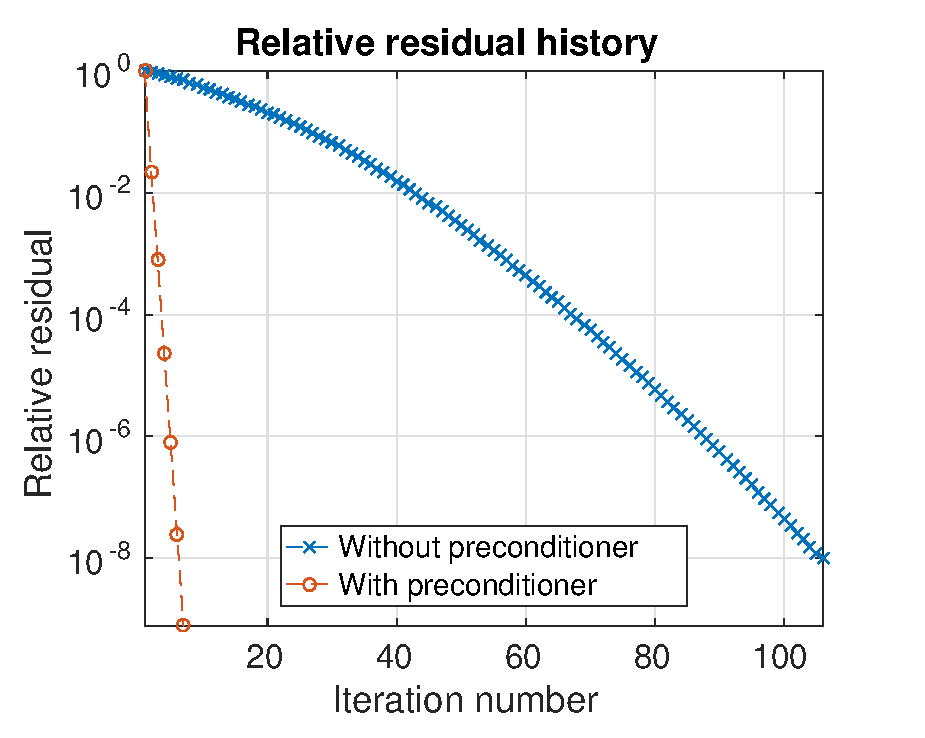
\includegraphics[scale=0.7]{PrecondLaplaceDirichletIterations}
	\caption{Number of iteration in the resolution of the single layer integral equation with a mesh of size $N = 500$.}
	\label{FigureNitLaplaceDirichlet}
\end{figure}


\subsection{Numerical results}

In this section, we provide some numerical results to accompany the previous analysis. 

\toDo{Inclure les figures d'ordre de convergence.}


\paragraph{}


\subsubsection{Convergence rates}
\subsubsection{Efficiency of the preconditioners}


\section{The case of the Helmholtz equation on a segment}

In tis section, we keep studying the flat segment $\Gamma = [-1,1]$, but tackle the non-zero frequency. Recall the definition of the single layer and hypersingular operators, $S_k$ and $N_k$, given in \eqref{defSk} and \eqref{defNk}, and the integral equations for the Dirichlet and Neumann problems, \eqref{Sklambda} and \eqref{Nkmu}. We introduce new preconditioners for the numerical resolution of those two equations that generalize the results of the previous section.  Let $S_{k,\omega} \isdef S_k \frac{1}{\omega}$ and $N_{k,\omega} \isdef N_k \omega$. We begin by establishing the following result:

\begin{The}
	\label{Commutations}
	The following commutations hold:
	\[S_{k,\omega} \left[-(\omega \partial_x)^2 - k^2\omega^2\right] =  \left[-(\omega \partial_x)^2 - k^2\omega^2\right]S_{k,\omega},\]
	\[N_{k,\omega} \left[-(\partial_x \omega)^2 - k^2\omega^2\right] =  \left[-(\partial_x \omega)^2 - k^2\omega^2\right]N_{k,\omega}.\]
	\begin{proof}
		We start with the first commutation. Since $(\omega \partial_x)^2$ is self adjoint and symmetric, we have 
		\[S_{k,\omega} (\omega \partial_x)^2 = \int_{-1}^{1} \frac{(\omega_y \partial_y)^2 \left[G_k(x-y)\right] u(y)}{\omega(y)},\]
		where we use the notation $\omega_y$ and $\partial_y$ to emphasize the dependence in the variable $y$. 
		Thus, 
		\[S_{k,\omega} (\omega \partial_x)^2 - (\omega \partial_x)^2 S_{k,\omega} = \int_{-1}^{1} \frac{D_k(x,y)u(y)}{\omega(y)},\]
		where $D_k(x,y) \isdef \left[(\omega_y \partial_y)^2 - (\omega_x \partial_x)^2\right] \left[G_k(x-y)\right]$. 
		One has 
		\[D_k(x,y) = G_k''(x-y) (\omega^2_y - \omega^2_x) + G_k'(x-y)(y + x).\]
		Since $G_k$ is a solution of the Helmholtz equation, we have for all $(x \neq y) \in \R^2$ 
		\[G_k'(x-y) = (y-x)(G_k''(x-y) + k^2G(x-y)),\]
		thus
		\[D_k(x,y) = G_k''(x-y)\left(\omega^2_y - \omega_x^2 + y^2 - x^2\right) + k^2(y^2 - x^2)G_k(x-y) . \]
		Note that $y^2 - x^2 = \omega_x^2 - \omega_y^2$ so the first term vanishes and we find
		\[S_{k,\omega} (\omega \partial_x)^2 - (\omega \partial_x)^2 S_{k,\omega} =  k^2\left(\omega^2 S_{k,\omega} -S_{k,\omega} \omega^2 \right). \]
		The proof of the second commutation is quite heavy and is postponed to annexes. 
	\end{proof}
\end{The}

This theorem shows that the operators $S_k$ and $N_k$ share the same eigenvectors as, respectively, $\left[-(\omega \partial_x)^2 - k^2\omega^2\right]$ and $ \left[-(\partial_x \omega)^2 - k^2\omega^2\right]$. We can look for eigenfunctions of the operator $\left[ -(\omega \partial_x)^2 - k^2\omega^2\right]$, to find a diagonal basis for $S_{k,\omega}$. They are the solutions to the differential equation 
\[ (1-x^2) y'' - x y' = \lambda y.\]
Once we set $x = \cos \theta$, $\tilde{y}(\theta) = y(x)$,  $q = \frac{k^2}{4}$, $a = \lambda + 2q$, $\tilde{y}$ is a solution of the standard Mathieu equation 
\[\tilde{y}'' + (a - 2q \cos(2\theta)) \tilde{y} = 0.\]
There are a discrete set of values $a_{2n}(q)$ for which this equation possesses an even and $2\pi$ periodic function. The corresponding solution is known as the Mathieu cosine, and usually denoted by $\textup{CE}_n$, with the normalization taken as
\[ \int_{0}^{2\pi} \textup{CE}_n(\theta)^2 d\theta = \pi.\]
Those functions satisfy 
\[ \int_{-\pi}^{\pi}\textup{CE}_n(\theta) \textup{CE}_m(\theta) = \pi \delta_{m,n},\]
thus, any even $2\pi$ periodic function in $L^2(-\pi,\pi)$ can be expanded along the functions $\textup{CE}_n$, with the coefficients obtained by orthonormal projection. Letting 
\[T_{n}^k \isdef \textup{CE}_n(\arccos(x),\]
in analogy to the zero-frequency case, we have
\[\left[-(\omega \partial_x)^2 - k^2\omega^2\right] T_{n,k} = \lambda_{n,k}^2 T_{n,k}.\]
For large $n$, using the general results from the theory of Hill's equations (see \cite[eq. 28.29.21]{NIST:DLMF}) we have the following asymptotic formula for $\lambda_{n,k}$:
\[ \lambda_{n,k}^2 = n^2 - \frac{k^4}{16n^2} +o \left(n^{-2}\right). \]
The first commutation established in \autoref{Commutations} implies that the Matthieu cosines are also the eigenfunctions of the single-layer operator. An equivalent statement is given in \cite[Thm 4.2]{betcke2014spectral} (see also references therein), if we allow the degenerate case $\mu = 0$. There, a decomposition of the Hankel kernel is given as a sum of products of the Mathieu Cosine, in close analogy to the decomposition of the logarithmic kernel stated in \autoref{decompLnKernelTn}. Unfortunately, the lack of explicit eigenvalues for $S_{k,\omega}$ prevents us from applying a similar analysis as that performed in the first part of this work. Instead, we will perform a perturbation analysis, much like \cite{bruno2012second}. 

\subsection{Dirichlet}

In this section, we focus on the Dirichlet problem with non-zero frequency, and the corresponding integral equation 
\begin{equation}
S_k \lambda = u_D
\label{Sklambda2}
\end{equation}
Here again, we define a rescaled operator $S_{k,\omega} \isdef S_k \frac{1}{\omega}$, i.e.
\[S_{k,\omega}\alpha : x \mapsto \int_{-1}^1 \dfrac{H_0(k|x-y|) \alpha(y)}{\omega(y)}dy.\]
If we let $\lambda = \dfrac{\alpha}{\omega}$, then equation \eqref{Sklambda2} is equivalent to
\[S_{k,\omega}\alpha = u_D.\]
The Hankel function can be written as 
\[H_0(z) = \frac{-1}{2\pi}\ln|z| J_0(z) + F_1(z^2)\]
where $J_0$ is the Bessel function of first kind and order $0$ and where $F_1$ is analytic. Using the power series definition of $J_0$, 
\begin{align}
	\begin{split}
		\frac{i}{4}H_0(k \abs{x - y}) &= \frac{-1}{2\pi}\ln |x-y| \label{decompHankel}\\ 
		&\quad + \frac{1}{2\pi} \frac{k^2}{4} (x- y)^2 \ln |x-y|\\
		&\quad + (x-y)^4 \ln|x-y|F_2(x,y) + F_3(x,y)
	\end{split}
\end{align}
\noindent where $F_2$ and $F_3$ are $C^{\infty}$. Let us study the operators $O_n$ defined for $n \geq 1$ as 
\[O_n : \alpha \mapsto \int_{-1}^{1}(x-y)^{n-1} \ln\abs{x - y} \frac{\alpha(y)}{\omega(y)}.\]

\begin{Lem}
	\label{lemPseudoDiffOn}
	For all $n \geq 1$, there exists a function $o_n : \N^2 \to \R$ satisfying the following conditions 
	\begin{itemize} \item[(i)] \itemequation[sumDefiningOn]{}{$	\forall k \in \Z, \quad O_n T_k = \displaystyle\sum_{i = -\infty}^{+\infty} o_n(k,i)T_{k-i}$}{}
	\item[(ii)] \itemequation[conditionon]{}{	$\forall \alpha, \beta \in \N, \forall  i,k  \in \Z, \quad  \abs{\Delta_i^\alpha \Delta_k^\beta o_n(k,i)} \leq C_{n,\alpha,\beta} (1 + k^2)^{-n - 1 - \beta}$}{} 
	\item[(iii)]\itemequation[conditionon]{}{$\forall i,k \in \Z, \quad \abs{i} \geq  n \implies o_n(k,i) = 0$}{}
	\end{itemize}
	where $\Delta_i$ and $\Delta_k$ represent the discrete derivation operator in the variables $i$ and $k$ respectively, e.g. 
	\[ \Delta_i o_n(k,i) = o_n(k,i+1) - o_n(k,i),\]
	and $\Delta_i^\alpha$ denotes the $\alpha$-th iterate of $\Delta_i$. We use the convention $T_k \isdef T_{\abs{k}}$ for $k \in \Z$. 
\end{Lem}
	\begin{proof}
		We shall prove this by induction. First for $n = 1$, $O_1 = 2\pi S_\omega$, and we simply have $o_1(k,i) = \delta_{i = 0} s_k$ where $s_k$ are the eigenvalues of $S_\omega$ defined in \autoref{STn}. Obviously, $o_1$ satisfies all the requirements. Second, notice that for $n \geq 1$, 
		\[O_{n+1} = x 0_n - O_n x,\]
		which combined with the identity 
		\[x T_n = \dfrac{T_{n-1} + T_{n+1}}{2}\]
		valid for all $n \in \Z$, implies
		\[O_{n+1}T_k = \sum_{i= -\infty}^{+\infty} o_n(k,i) \dfrac{T_{k - i + 1} + T_{k _-i- 1}}{2} - \frac{1}{2} O_n T_{k+1} - \frac{1}{2} O_n T_{k - 1}.\]
		By the recurrence assumption (i), this implies 
		\begin{eqnarray*}
			O_{n+1}T_k &=& \frac{1}{2} \sum_{-\infty}^{+ \infty}\left(o_n(k,i-1) - o_n(k+1,i - 1)\right) T_{k - i} \\
			&&+ \frac{1}{2} \sum_{-\infty}^{+ \infty}\left(o_n(k,i+1) - o_n(k-1,i + 1)\right) T_{k - i}.
		\end{eqnarray*}
		Thus, condition (i) is satisfied with 
		\[o_{n+1}(k,i) \isdef \frac{\left(o_n(k,i-1) - o_n(k+1,i-1) + o_n(k,i+1) - o_n(k-1,i+1)\right)}{2}.\]
		If $\abs{i} \geq n+1$ then by triangular inequality $\abs{i-1} \geq n$ and $\abs{i+1} \geq n$ so all terms in the rhs are null by the assumption (iii), which shows that (iii) also holds for $o_{n+1}$. Finally, the assumption (ii) is easily checked for $o_{n+1}$ once we write 
		\[ o_{n+1}(k,i) = \frac{- \Delta_k(k,i-1) + \Delta_k(k-1,i+1)}{2}.\]
	\end{proof}


\begin{Lem}
	\label{orderOfOn}
	The operator $O_n$ is of order $n$. 
\end{Lem}
\begin{proof}
	Since the sum in \eqref{sumDefiningOn} is finite, by linearity, it is sufficient to show that the operator $O^i_n$ defined by 
	\[ \forall k \in \Z, \quad  O^i_n T_k = o_n(k,i) T_{k-i} \]
	is of order $n$. We treat the case $i > 0$, the opposite case being analogous. Let $u \in T^s$ for some $s$, there holds 
	\[ O^i_n u = \sum_{k = 0}^{+ \infty} o_n(k + i,i)\hat{u}_{k + i}T_k + \sum_{k = 0}^{i} o_n(i - k,i) \hat{u}_{i - k}T_k\]
	which we rewrite $O_n^i u = Vu + Ru$. Obviously, $R$ is a smoothing operator with
	\[ \norm{Ru}_{T^{s + n}} \leq (1 + i)^{n} \norm{u}_{T^s}.\]
	Now, for all $k \in \N$ let
	\[\hat{v}_k \isdef o_n(i + k,i) \hat{u}_{i + k}.\]
	Applying Peetre's inequality, one has
	\[(1 + k^2)^{n + s}\abs{\hat{v}_k}^2 \leq C \left(1 + i^2\right)^{\abs{n + s}}\left(1 + (i + k)^2\right)^{n + s} \abs{o_n(k + i,i)}^2 \abs{\hat{u}_{k+i}}^2.\]
	the condition (ii) in \autoref{lemPseudoDiffOn} with $\alpha = \beta = 0$ yields
	\[\abs{o_n(k+i,i)}^2 \leq C\left(1 + (k+i)\right)^{-2n} \leq 2C \left(1 + (k+i)^2\right)^{-n}.\]
	Therefore, $\norm{V u}_{T^{s + n}} \leq C(1 + i)^{\abs{n + s}} \norm{u}_{T^s}$ which concludes the proof. 
\end{proof}
\begin{Cor}
	The operator $S_{k,\omega}$ admits the following expansion 
	\[ S_{k, \omega} = S_\omega + \frac{1}{2\pi} \frac{k^2}{4} O_3 +  R_5 + R_{\infty}\]
	\label{developpementHankel}
	where $R_5$ is an operator of order $5$ and $R_\infty$ is a smoothing operator.
\end{Cor}
\begin{proof}
	From equation \eqref{decompHankel}, it suffices 
\end{proof}
In particular, the operator $S_{k,\omega}$ is well defined on $T^{-\infty}$, and is of order $1$.

The expansion obtained in \autoref{developpementHankel} together with the previous lemma imply the following
\begin{The} There holds:
	\[S_{k,\omega}  (\omega\partial_x)^2 S_{k,\omega} = \frac{I}{4} + K\]
	where $K$ is of order $2$. 
\end{The}

In fact, we will show a more precise result, that includes the first correction due to frequency number:
\begin{The} There holds
	\label{TheHelmholtz}
	\[S_{k,\omega} \left( -(\omega \partial_x)^2 - k^2\omega^2\right) S_{k,\omega} = \frac{I}{4} + K'\]
	where $K'$ is of order $4$. 
	\begin{proof}
		Using the expansion of \autoref{developpementHankel}, we can write 
		\begin{eqnarray*}
			-S_{k,\omega}(\omega \partial_x)^2 S_{k,\omega} &=& -S_\omega (\omega \partial_x)^2 S_\omega \\
			&& - \frac{1}{2\pi}\frac{k^2}{4}\left(S_\omega (\omega \partial_x)^2 O_3 + O_3 (\omega \partial_x)^2 S_\omega\right) + K'
		\end{eqnarray*}
		where $K'$ is of order $4$. By \autoref{TheSdx2S}, the first term is $\frac{I}{4} + R$ where $R$ is a smoothing operator. Then, simple calculations show that
		\[(\omega \partial_x)^2 \left((x - y)^2\ln|x-y|\right) = 2 \omega^2(x)\ln|x-y| -2x(x-y) \ln|x-y| + P(x,y)\]
		where $P$ is a polynomial in $x$ and $y$. Dividing by $\omega(y)$ and integrating on both sides with respect to $y$, we get 
		\[\frac{1}{2\pi}(\omega \partial_x)^2 O_3 = 2 \omega^2 S_\omega - \frac{1}{\pi}xO_2 + R \]
		where $R$ is a smoothing operator. Taking the adjoint operator in both sides (with respect to the $T^0$ scalar product), we get
		\[\frac{1}{2\pi}O_3(\omega \partial_x)^2 = 2 S_\omega\omega^2 + \frac{1}{\pi}O_2x + R'\]
		where $R'$ is also a smoothing operator. \autoref{orderOfOn} thus implies
		\[-S_{k,\omega}(\omega \partial_x)^2 S_{k,\omega} = \frac{I}{4} - k^2S_\omega \omega^2 S_\omega + K''\]
		where $K''$ is of order $4$.
		The announced result holds since, using \autoref{developpementHankel}, 
		\[S_\omega \omega^2 S_\omega - S_{k,\omega} \omega^2 S_{k,\omega}\]
		is an operator of order $4$.
	\end{proof}
\end{The}


\toDo{Reporter ça après le non flat arc, puis parler du cas courbe fermée et poids $\omega = 1$ avec l'analogie Darbas Antoine.}
The last result, when also in consideration of the commutation shown in \autoref{Commutations}, implies that $\sqrt{ -(\omega \partial_x)^2 - k^2\omega^2}$ is a compact perturbation of the inverse of $S_{k,\omega}$, prompting us to use it as a preconditioner in Equation \eqref{Sklambda2}.

\section{Non-flat arc, Helmholtz}

\begin{itemize}
	\item[-] Restate the theorem, en disant que c'est la même preuve. 
\end{itemize}

We return to the case of a $C^{\infty}$ non-intersecting open curve $\Gamma$ and non-zero frequency $k$, and define a new preconditioner for thee corresponding integral equation. The main result of this section is \autoref{TheHelmholtz} We fix a smooth, constant speed, parametrization $r : [-1,1] \to \mathbb{R}^2$ of $\Gamma$. The constant-speed assumption ensures $(x,y) \in [-1,1]$, one has
\begin{equation}
\abs{r(x) - r(y)^2} = \frac{\abs{\Gamma}^2}{4} \abs{x - y}^2 + |x-y|^4 F_1(x,y)
\label{DLcourbe_param}
\end{equation}
where $\abs{\Gamma}$ is the length of $\Gamma$ and $F_1$ is a $C^{\infty}$ function on $[-1,1]^2$.


\subsection{Neumann}

\subsection{Numerical results}


\section{Conclu}

Résumé de ce qu'on a fait, du lien qu'on a fait. Ouverture sur les singularités de type coin puis 3D. Beaucoup plus compliqué car pas de relations analytiques qui nous aident. 
Expliquer la beauté de l'approche numérique avec un poids. On propose le préconditioneur avec un test numérique ? 

Possible analyse pseudo-diff ? En reparler ? Lien avec Antoine et Darbas. 

\section{Commutation of $N_\omega$ and $(\partial_x \omega)^2 + k^2\omega^2$}

To ease the computations, we take some notations: let $\Delta_\omega \isdef (\omega \partial_x)^2$, $\Delta_\omega^T \isdef (\partial_x \omega)^2$,  $N_\omega \isdef N_{k,\omega}$, and $S_\omega \isdef S_{k,\omega}$. Using, \autoref{NkenfonctiondeSk} we can write 
\[N_\omega = -\partial_x S_\omega \omega \partial_x \omega - k^2 S_\omega \omega^2.\]
To show that $N_\omega$ and $\Delta_\omega^T + k^2\omega^2$ commute, we compute their commutator $C$ and show that it is null. 
We have 
\begin{eqnarray*}
	C &\isdef& N_\omega \Delta_\omega^T - \Delta_\omega^T N_\omega + k^2N_\omega \omega^2 - k^2 \omega^2 N_\omega \\
	&=& -\partial_x S_\omega \Delta_\omega \omega \partial_x \omega  - k^2 S_\omega \omega^2 \Delta_\omega^T \\
	&& + \partial_x \Delta_\omega S_\omega \omega \partial_x \omega + k^2 \Delta_\omega^T S_\omega \omega^2 \\
	&& - k^2 \partial_x S_\omega \omega \partial_x \omega^3 - k^4 S_\omega \omega^4 \\
	&& + k^2 \omega^2 \partial_x S_\omega \omega \partial_x \omega + k^4 \omega^2 S_\omega \omega^2
\end{eqnarray*}
where each term in the r.h.s. of the first equality gives rise to a line in the second. We rearrange the terms as follows:
\begin{eqnarray*}
	C &=& \partial_x (\Delta_\omega S_\omega - S_\omega \Delta_\omega) \omega \partial_x \omega - k^2 \partial_x S_\omega \omega \partial_x \omega^3 + k^2 \omega^2 \partial_x S_\omega \omega\partial_x \omega\\	
	&& + k^4 (\omega^2 S_\omega - S_\omega \omega^2) \omega^2\\
	&& + k^2(\Delta_\omega^T S_\omega \omega^2 - S_\omega \omega^2 \Delta_\omega^T)
\end{eqnarray*}
For the first term, we inject the commutation shown in \autoref{Commutations}. For the last line, we use the following identities: 
\[ \Delta_\omega^T = \Delta_\omega - 2x \partial_x - 1\]
\[ \omega^2 \Delta_\omega^T = \Delta_\omega \omega^2 + \omega^2 + 2 \omega x \partial_x \omega\]
Let $D = \frac{C}{k^2}$, 
\begin{eqnarray*}
	D &=& \partial_x S_\omega \omega (\omega^2\partial_x - \partial_x \omega^2) \omega  + (\omega^2 \partial_x - \partial_x \omega^2)S_\omega \omega \partial_x \omega\\
	&&+ k^2(\omega^2 S_\omega - S_\omega \omega^2) \omega^2\\
	&&+ (\Delta_\omega - 2x \partial_x - 1)S_\omega \omega^2 - S_\omega(\Delta_\omega \omega^2 + \omega^2 + 2\omega x \partial_x \omega) 
\end{eqnarray*}
We use $\omega^2 \partial_x - \partial_x \omega^2 = 2x$, and the relation $\partial_x S \omega^2 = S_\omega \omega \partial_x \omega$, obtained by integration by parts. 
\begin{eqnarray*}
	D &=& 2 S_\omega \omega \partial_x x\omega + 2 x S_\omega  \omega \partial_x \omega \\
	&& + \left(k^2(\omega^2 S_\omega - S_\omega \omega^2) + \Delta_\omega S_\omega - S_\omega \Delta_\omega \right)\omega^2\\
	&& - 2 S_\omega \omega^2 - 2 x  S_\omega \omega \partial_x \omega - 2 S_\omega \omega x \partial_x \omega
\end{eqnarray*}
Using again the commutation shown in \autoref{Commutations}, we are left with 
\begin{eqnarray*}
	D &=&  2 S_\omega \omega (\partial_x x - x \partial_x) \omega - 2 S_\omega \omega^2
\end{eqnarray*}
This is null since $\partial_x x - x \partial_x = 1$. 

\section{Plus}











\bibliographystyle{plain}
\IfFileExists{biblio.bib}{\bibliography{biblio}}{\bibliography{/home/emile/Documents/Martin/Thesis/Biblio/biblio.bib}}


\end{document}


